% !TEX encoding = UTF-8 Unicode
% !TEX TS-program = pdflatex

%%%%%%% La riga soprastante serve per configurare gli editor
%%%%%%% TeXShop, TeXworks e TeXstudio per gestire questo file
%%%%%%% con la codifica UFF-8.
%%%%%%% Se si vuole usare un'altra codifica si veda sotto.
%%%%%%%

%%%%%%%  Esempio con molte opzioni
%%%%%%% Le opzioni nella forma "chiave=valore" sono definite
%%%%%%% perché la classe dalla versione 6.1.00 usa il pacchetto
%%%%%%% xkeyval. Vedere sulla documentazione in inglese o
%%%%%%% in italiano quali chiavi accettano valori.

%%%%%%% L'opzione per il corpo accetta qualsiasi valore, anche fratto
%%%%%%% (per esempio: corpo=11.5pt) e va sempre scritto con una
%%%%%%% unità di misura. L'utente è pregato di non esagerare con
%%%%%%% corpi normali minori di 9.5pt o maggiori di 13pt.
%%%%%%%
%%%%%%% Le opzioni per inputenc e fontenc vanno per prime.
%%%%%%% Vengono ignorate se NON si compone con pdfLaTeX. Ma
%%%%%%% questo è un esempio per pdfLaTeX.
%%%%%%%

\documentclass[%
    corpo=12pt,
    twoside,
    stile=classica,   
% 	oldstyle,
%   autoretitolo,
    tipotesi=magistrale,
    evenboxes,
    english,
%	cucitura=7mm,
	numerazioneromana,
]{toptesi}
%%%%%%%%%%%%%%%%%%%%%%%%%%%%%%%%%%%%%%%%%%%%%%%%%%%%
%%%%%% Per la codifica d'entratasi può scegliere quella che si vuole,
%%%%%% ma si consiglia di preferire utf8; in ogni caso non scegliere
%%%%%% codifiche specifiche del sistema operativo.

\usepackage[utf8]{inputenc}% codifica d'entrata
\usepackage[T1]{fontenc}%    codifica dei font
\usepackage{lmodern}%        scelta dei font

% Vedere la documentazione toptesi-it.pdf per le
% attenzioni che bisogna usare al fine di ottenere un file
% veramente conforme alle norme per l'archiviabilità.
% \usepackage{imakeidx}
\begin{pdfxmetadata}
	\Title{Approaches for Domain Adaptive Object Detection in Production Environments}
	\Author{Gabriele Degola}
	\Publisher{Politecnico di Torino}
	\Keywords{domain adaptation\sep
	object detection\sep
	computer vision\sep
	machine learning\sep
	sim2real}
\end{pdfxmetadata} 
\usepackage[a-1b]{pdfx}

% \usepackage[hidelinks]{hyperref}

\hypersetup{%
	hidelinks,
    pdfpagemode={UseOutlines},
    bookmarksopen,
    pdfnewwindow=true,
    pdfstartview={FitH}
}
%
%%%%%%% Esempio di composizione di tesi di laurea con PDFLATEX 
%
\usepackage{amssymb}
\usepackage{csquotes}
\usepackage{lipsum}
\usepackage{subcaption}
\usepackage{biblatex}
\addbibresource{references.bib}
\usepackage[acronym]{glossaries}
\usepackage{tabularx}
\usepackage{multirow}
\usepackage{xurl}
\usepackage{nicematrix}
\usepackage{nicefrac}
\usepackage{booktabs}
\usepackage{epigraph}

\usepackage[
	type={CC},
	modifier={by-nc-sa},
	version={4.0},
	lang={english}
]{doclicense}
%

\makeglossaries
\newacronym{ai}{AI}{artificial intelligence}
\newacronym{ilsvrc}{ILSVRC}{ImageNet Large Scale Visual Recognition Challenge}
\newacronym{cnn}{CNN}{convolutional neural network}
\newacronym{resnet}{ResNet}{residual neural network}
\newacronym{gan}{GAN}{generative adversarial network}
\newacronym{svm}{SVM}{Support Vector Machines}
\newacronym{knn}{KNN}{K-Nearest Neighbors}
\newacronym{ide}{IDE}{Integrated Development Environment}
\newacronym{iou}{IoU}{Intersection over Union}
\newacronym{roc}{ROC}{Receiver Operating Characteristic}
\newacronym{auc}{AUC}{Area Under the Curve}
\newacronym{ap}{AP}{Average Precision}
\newacronym{map}{mAP}{mean Average Precision}
\newacronym{json}{JSON}{JavaScript Object Notation}
\newacronym{xml}{XML}{Extensible Markup Language}
\newacronym{voc}{VOC}{Visual Object Classes}
\newacronym{kitti}{KITTI}{Karlsruhe Institute of Technology and Toyota Technological Institute}
\newacronym{rcnn}{R-CNN}{region-based convolutional neural network}
\newacronym[firstplural=Regions of Interest (RoIs)]{roi}{RoI}{Region of Interest}
\newacronym{rpn}{RPN}{Region Proposal Network}
\newacronym[first=\textit{Feature Pyramid Network} (FPN)]{fpn}{FPN}{Feature Pyramid Network}
\newacronym[first=\textit{non-maximum suppression} (NMS)]{nms}{NMS}{non-maximum suppression}
\newacronym{ssd}{SSD}{Single Shot Detector}
\newacronym{yolo}{YOLO}{You Only Look Once}
\newacronym{adda}{ADDA}{Adversarial Discriminative Domain Adaptation}
\newacronym{dann}{DANN}{Domain Adversarial Neural Network}
\newacronym{coco}{COCO}{Common Objects in Context}
\newacronym[firstplural=GPUs]{gpu}{GPU}{Graphics Processing Unit}
\newacronym{cpu}{CPU}{Central Processing Unit}
\newacronym[first=\textit{multi-layer perceptron} (MLP)]{mlp}{MLP}{multi-layer perceptron}
\newacronym{relu}{ReLU}{rectified linear unit}
\newacronym{sift}{SIFT}{scale-invariant feature transform}
\newacronym{hog}{HOG}{histogram of oriented gradients}
\newacronym{pca}{PCA}{Principal Component Analysis}
\newacronym{lpips}{LPIPS}{Learned Perceptual Image Patch Similarity}

\glsdisablehyper

%%%%%%% Definizioni locali
%\newtheorem{osservazione}{Osservazione}% Standard LaTeX
\ExtendCaptions{english}{Abstract}{Acknowledgements}
\newcommand{\quotes}[1]{``#1''}


\begin{document}
\english
%%%%%%% Questi comandi è meglio metterli dentro l'ambiente
%%%%%%% ThesisTitlePage con o senza asterisco, oppure in un file di
%%%%%%% configurazione personale. Si veda la documentazione
%%%%%%% inglese o italiana.
%%%%%%% Comunque i presenti comandi servono per comporre la
%%%%%%% tesi con i moduli di estensione standard del pacchetto
%%%%%%% TOPtesi.

\begin{ThesisTitlePage}*
\ateneo{Politecnico di Torino}% nome generico dell'Universita'
%\nomeateneo{Weiss Turm}% eventuale nome proprio dell'universita'
\logosede[4cm]{logopolito}% logo dell'universita'
\FacoltaDi{DEPARTMENT OF\space}% Etichetta della facolta'
\facolta{CONTROL AND COMPUTER ENGINEERING}% facolta'
%\Materia{Remote sensing}
%\titolo{Domain Adaptation for Object Detection}% 
\titolo{Approaches for Domain Adaptive Object Detection in Production Environments}% 
%\sottotitolo{A data augmentation approach}% 
\CorsoDiLaureaIn{Master of Science in\space}
\corsodilaurea{Data Science and Engineering}% per la laurea
\TesiDiLaurea{Master Thesis}
\def\Candidato{Candidate}
%\candidato{Gabriele \textsc{Degola}}[273479]% per tutti i percorsi 
\candidato{Gabriele \textsc{Degola}}% per tutti i percorsi 
\AdvisorName{Supervisor}
\relatore{prof.~Paolo \textsc{Garza}}% per la laurea e/o il dottorato
%\secondorelatore{prof.~Olivier François}
%\relatore{{\tabular[t]{@{}l}
%		prof.~Paolo \textsc{Garza}\\
%		\qquad\small{Politecnico di Torino}\\[0.5ex]
%		prof.~Olivier \textsc{François}\\
%		\qquad\small{Grenoble INP - Ensimag}
%		\endtabular}
%}
\tutoreaziendale{dr.~Etienne \textsc{Balit}\\ing.~Valérian \textsc{Gonnot}}
\NomeTutoreAziendale{Company advisors\\Neovision}

\sedutadilaurea{\textsc{April 2022}}% per la laurea magistrale
\end{ThesisTitlePage}

%\pagenumbering{roman}
\vspace*{\fill}
\doclicenseThis
%\paginavuota

\sommario
Nowadays, computer vision is built almost exclusively on deep learning methods. Research in recent years has improved more and more the performances of convolutional neural networks on several popular key tasks, such as image classification, detection and segmentation. However, these methods require large amounts of annotated data to be trained effectively, which are not always available.

For this reason, domain adaptation methods have been widely studied and developed. The goal is to transfer the knowledge learned by a machine learning model on annotated data to data from other domains for which annotations are not available or only partially. A typical case is the transfer from synthetic data (easy to generate in large quantities) to real data (expensive to collect and annotate).

\bigskip
This work focuses on domain adaptation for an object detection task, with the goal of identifying methods that can be deployed in production environments. It starts from a review of both the fundamental and some recently proposed methods and explores a simple approach to domain adaptation, without the need for complex modifications to the most commonly used network architectures. At the same time, it attempts to address some issues of more popular domain adaptation methods for object detection, that may hinder their use in actual applications.

The performed experiments show that the method can be easily applied by engineers for satisfactory results in real world projects, when it is complex to obtain image annotations.

\paginavuota % funziona anche senza specificare l'opzione classica

\ringraziamenti
\begin{otherlanguage*}{italian}
\makebox[\textwidth][r]{
	\begin{minipage}[t]{.45\textwidth}
		\large{\textit{Alla mia famiglia\\Ad Alba\\Ai miei nonni}}
	\end{minipage}
}
\end{otherlanguage*}

\vspace*{1cm}

\bigskip
\foreignlanguage{french}{Merci à Valérian, Etienne, Olivier, Taiamiti et à tout le monde chez Neovision, pour m'avoir accueilli comme si je faisais partie de l'équipe et pour m'avoir suivi minutieusement et patiemment tout au long de mon stage.}

\bigskip
I would like to sincerely thank the supervisor of this work, professor Paolo Garza, for his thorough revision and for the useful comments and advice.

\bigskip
Thanks to the great people I have come across over these years. It has been a fun journey.

%\newpage
\paginavuota

\iffalse
\begin{dedica}
	Alla mia famiglia\\
	Ad Alba\\
	Ai miei nonni
\end{dedica}
\fi

\english

\iffalse
\begin{citazioni}
	\textit{\quotes{So, nobody told me what to do\\~And there was no preconception of what to do.}}
	
	---Giorgio Moroder
\end{citazioni}
\fi

\vspace*{1cm}
\renewcommand{\epigraphsize}{\normalsize}
\setlength{\epigraphwidth}{0.56\textwidth}
\renewcommand{\sourceflush}{flushright}
\let\originalepigraph\epigraph 
\renewcommand\epigraph[2]{\originalepigraph{\textit{#1}}{\textsc{#2}}}
\epigraph{Once you free your mind about a concept of\\Harmony and of music being \quotes{correct},\\You can do whatever you want.\\So, nobody told me what to do\\And there was no preconception of what to do.}{--- Giorgio Moroder}

\paginavuota

%\tablespagetrue\figurespagetrue % normalmente questa riga non serve ed e' commentata
%\setcounter{tocdepth}{1}
\indici
%\paginavuota

\mainmatter
\english
%\pagenumbering{arabic}

\phantomsection
\chapter*{Introduction}
\addcontentsline{toc}{chapter}{Introduction}
Over the past few decades, machine learning and deep learning techniques have achieved impressive results in a variety of tasks, of which computer vision and language processing are probably the best known. However, they generally assume that training and inference data are drawn from the same distribution, which is not always the case. Furthermore, data collection and annotation is an expensive and time-consuming task. It may therefore be desirable to apply a model trained on annotated data to another domain for which annotations are not available or only partially available. Several methods have been proposed to reduce the domain shift between the two data distributions. They have been widely studied and are presented in the following sections.

\bigskip
The starting point of this Master Thesis is a six-months internship carried out at Neovision\footnote{\url{https://neovision.fr/en/}}, an engineering company based in Grenoble, France, and specialized in artificial intelligence. Transferring knowledge between different domains in an object detection scenario is a captivating but challenging task with applications in a variety of domains of great commercial interest. In addition, the shortage of available annotated data for the use case of interest is often one of the biggest obstacles for machine learning projects: engineers have to spend several hours gathering and possibly annotating related data, rather than focusing on algorithms and optimization. On the other hand, synthetic data can be easily generated in large quantities.

In addition, the tasks at hand can frequently be similar, but with data collected under different conditions of brightness, light spectrum, camera angle, and more. Previously trained models cannot be reused, and long training processes are therefore required. This is why Neovision is interested in tackling the domain adaptation problem, in order to offer the acquired knowledge and methods to its numerous customers. For this reason, the research documented in this Master Thesis proposes and shows that simple approaches for domain adaptive object detection, independent of specific employed network architectures and without introducing complex architecture modifications, can obtain satisfactory results and compete with more challenging methods previously proposed in the literature.


\chapter{Problem definition}
\section{Neural networks and computer vision}
Thanks to their achievements in computer vision, deep learning methods based on \glspl{cnn} have aroused a lot of interest over the last decade and have been used in many other branches of artificial intelligence. \Glspl{cnn} are a class of artificial neural networks, designed for the processing of structured arrays of data such as images.

\subsection{Machine learning}
The goal of machine learning is to extract patterns from raw input data, making a computer program build its own knowledge without relying on any hard-coded expertise. This knowledge is built from some representative data for the task of interest (the \textit{training set}) in order to make predictions or take decisions on new data that may only be available over time (the \textit{test set}). Machine learning approaches are often organized in three broad categories:

\begin{itemize}
	\item \textbf{Supervised learning}, in which training data are provided as input-output pairs and the goal is to learn a rule that maps the inputs to the outputs. Common supervised learning problems are classification, when the response variable belongs to a discrete set, and regression, in which the objective is to estimate a continuous mapping function.
	\item \textbf{Unsupervised learning}, in which patterns and similarities in the data are sought without the need of data labels.
	\item \textbf{Reinforcement learning}, in which the computer program (called \textit{agent}) interacts with an unknown environment and records the rewards associated to the actions it takes, progressively discovering the environment. The objective is to learn sequences of actions that lead to reward maximization.
\end{itemize}

Popular supervised machine learning algorithms, such as \gls{svm} and \gls{knn}, have strong theoretical properties and have matched human performances on numerous tasks.

\begin{figure}[ht]
	\centering
	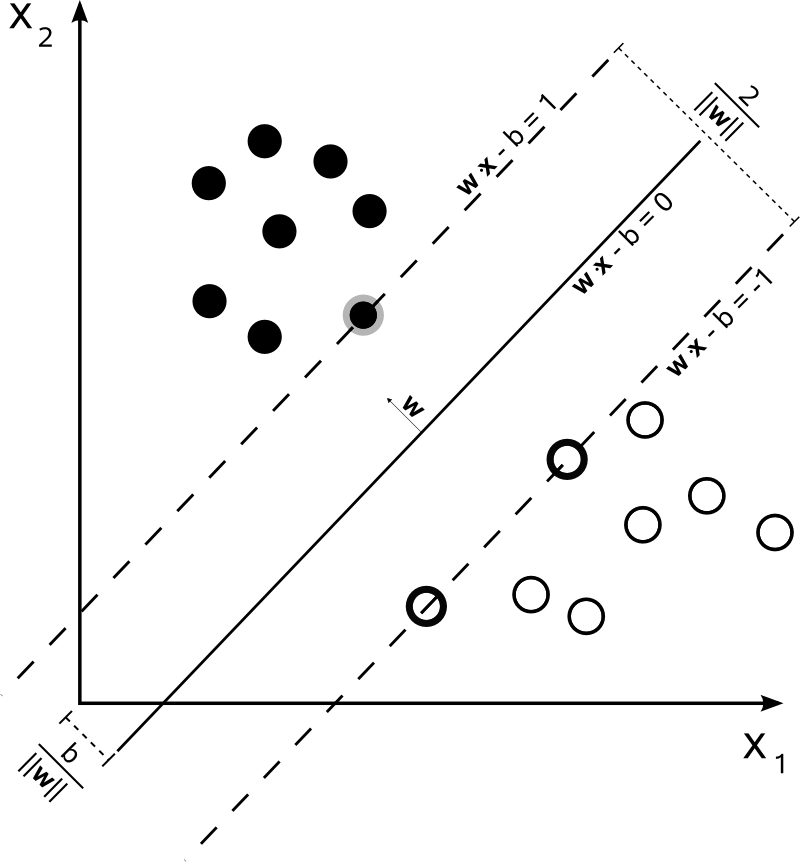
\includegraphics[width=.45\linewidth]{imgs/svm.png}
	\caption{\Gls{svm} for binary classification}
	\label{fig:supervised}
\end{figure}

%deep learning vs machine learning
%why we need cnn? images as structured output
\subsection{Deep learning}
Performances achieved by traditional machine learning algorithms heavily depend on the representation of the data with which they are fed. Indeed, they cannot analyze the full world, but only some pieces of relevant information that are available and used for learning. Each piece of information in the training examples is called a \textit{feature}. Traditional machine learning algorithms learn from these features, but cannot influence how they are defined and extracted from the real world data.

\medskip
Plenty of tasks can be solved by designing an appropriate set of features to extract, that will be forwarded to a machine learning algorithm. This requires previous knowledge, which is not always available, and intensive work and research from human actors. In many cases, it is extremely difficult to know a priori which features should be extracted. A clear example is dealing with images: humans can immediately distinguish a dog from a cat, but the difference in, e.g., fur and shape is not easy to describe in mathematical terms. A dog or a cat can take several poses and be pictured in various weather and lightning conditions. In addition, dogs or cat of different breeds can have very different appearance (high \textit{intra-class variation}) and sometimes have common traits with other animals (low \textit{inter-class variation}), but humans have no difficulty in classifying them as dogs or cats nevertheless. This makes the task complicated for machines.

\begin{figure}[ht]
	\centering
	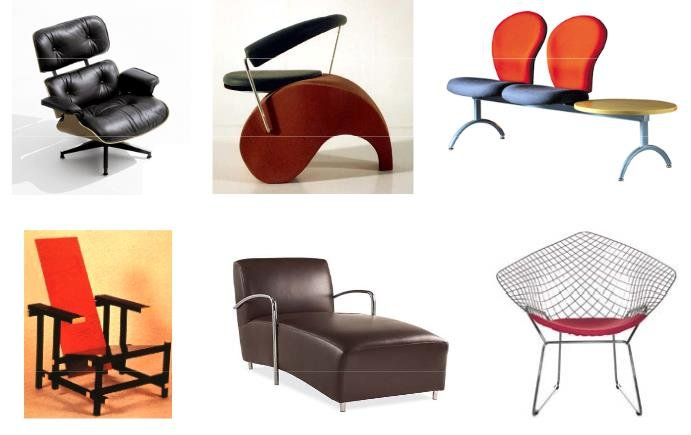
\includegraphics[width=.75\linewidth]{imgs/chairs.png}
	\caption{A popular example of \textit{intra-class variation}: even though they look different, humans do not have any trouble in saying all the images contain chairs.}
	\label{fig:intraclass}
\end{figure}

To solve the problem, it is possible to use machine learning to learn an effective data representation in addition to the mapping from inputs to outputs, an approach known as \textbf{representation learning}. This increases performances with respect to hand-crafted features and enables the algorithm to easily adapt to new tasks. However, not all extracted features may be useful to understand which animal is present in an image, while some of them can be sound only if considered together with other features.

\bigskip
\textbf{Deep learning} has been a fundamental milestone in representation learning. In deep learning, representations are expressed in terms of other simpler representations that were previously extracted from the input data. In the case of dog images, a \textit{deep neural network} can represent the concept of dog in terms of simpler concepts, such as corners and contours, which are in turn defined in terms of edges.

\begin{figure}[ht]
	\centering
	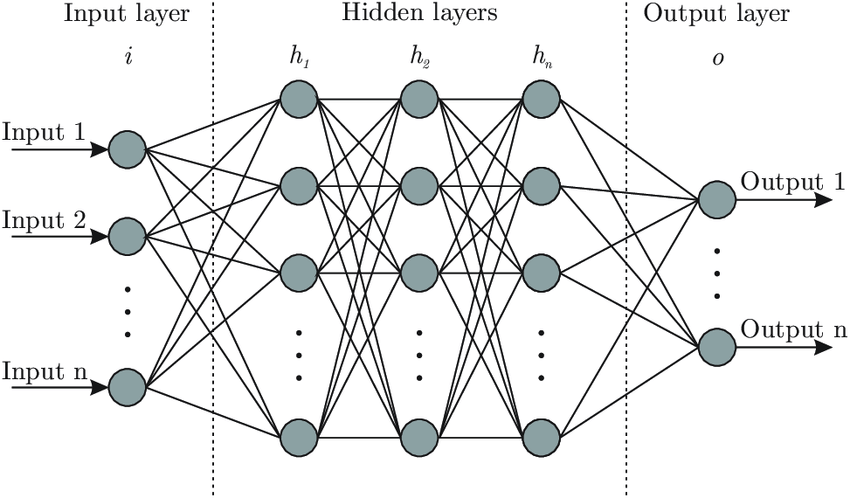
\includegraphics[width=.7\linewidth]{imgs/mlp.png}
	\caption{Example of feedforward neural network}
	\label{fig:mlp}
\end{figure}

\medskip
Different network architectures have been proposed for different tasks. The basic model is the \textit{feedforward neural network} or \gls{mlp}, whose schema is reported in Figure~\ref{fig:mlp}. Each node of the directed acyclic graph represents a neuron (from which the name \textit{neural network}): the first network layer is the input layer, with as many neurons as input features, while the last layer is the output layer, with one node for any class the network is designed to predict (or a single node in the case of binary classification). The intermediate layers are the hidden layers, in which every neuron computes the value of a linear function of the features returned by the previous layer, followed by a scalar non-linearity. Each output serves as input for all nodes in the next layer.

\bigskip
More formally, the output of the $j$\textsuperscript{th} node of the first hidden layer $h_1$, when receiving an observation $x$ from the $n$ input nodes, is the composition of:
\begin{itemize}
	\item a dot product $a_j$ between $x$ and the node's weight vector $w_j$, considering its bias term $b_j$:
	\begin{equation*}
		a_j = b_j + \sum_{i=0}^n w_{j,i}x_i
	\end{equation*}
	\item and a differentiable activation function $h$, such that:
	\begin{equation*}
		z_j = h(a_j)\text{.}
	\end{equation*}
\end{itemize}
This is incrementally repeated for all neurons of every network layer, until an output is produced by the neurons of the output layer. The network learns the weights $w$ associated to all neurons as well as their biases $b$, which define the output of the nodes when no input is provided\cite{amini2015apprentissage}.

\bigskip
Several activation functions have been proposed over the years to build deep neural networks and effectively exploit their depth. \textit{Sigmoid} and \textit{tan-h}, respectively defined as $h(t) = \nicefrac{1}{1 + e^{-t}}$ and $h(t) = \tanh(t) = \nicefrac{e^t - e^{-t}}{e^t + e^{-t}}$, have often been used as activation functions, as they squeeze input values to finite intervals ($[0,1]$ and $[-1,1]$ respectively, as represented in Figures~\ref{fig:sigmoid} and~\ref{fig:tanh}) and are biologically inspired. In modern deep learning, the default recommendation is to use the \gls{relu} function, defined as $h(t) = \max(0,t)$. With respect to sigmoid and tan-h, the \gls{relu} does not saturate (mitigating the risk of \textit{vanishing gradient}) and has faster convergence. An alternative is the \textit{leaky \gls{relu}}, defined as $h(t) = \max(\alpha t, t),\ \alpha \in [0,1]$, which in turn mitigates the risk of \quotes{dying} neurons, due to the fact that \gls{relu} sets all negative values to $0$.

\begin{figure}
	\centering
	\subcaptionbox{Sigmoid\label{fig:sigmoid}}{
		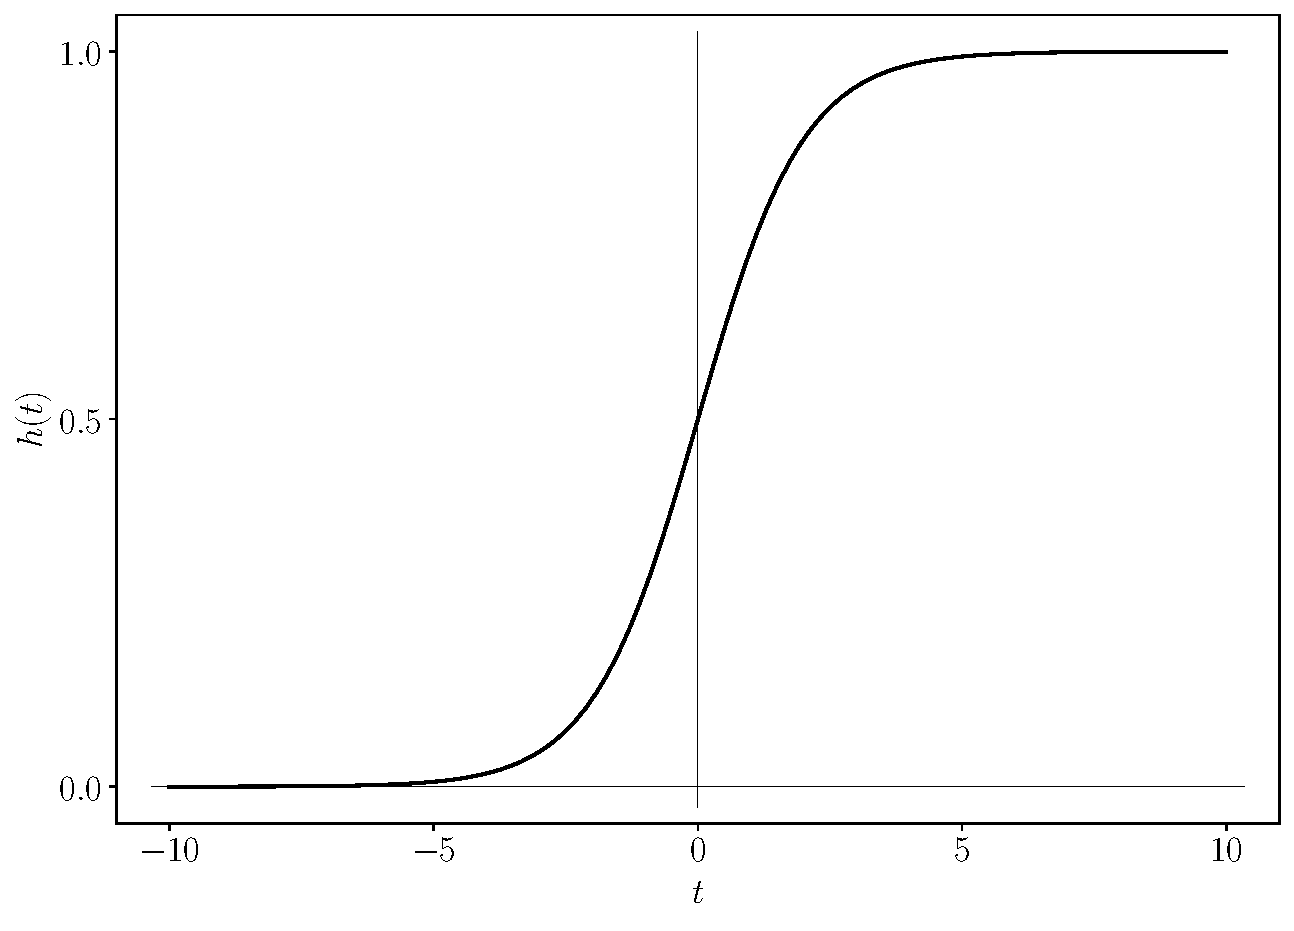
\includegraphics[width=.47\linewidth]{imgs/sigmoid.pdf}
	}
	\subcaptionbox{tan-h\label{fig:tanh}}{
		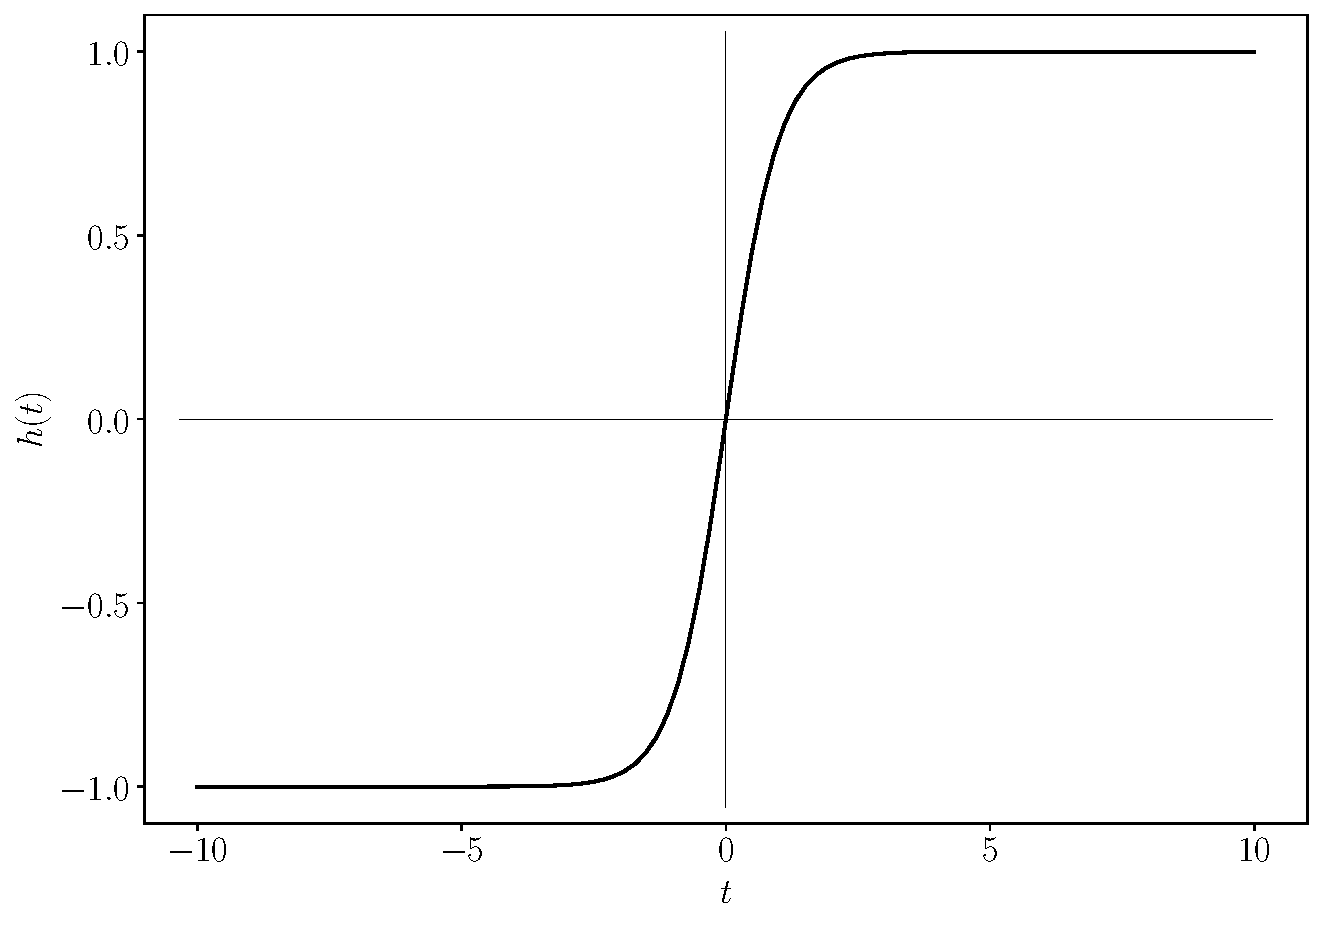
\includegraphics[width=.47\linewidth]{imgs/tanh.pdf}
	}\\
	\subcaptionbox{\gls{relu}}{
		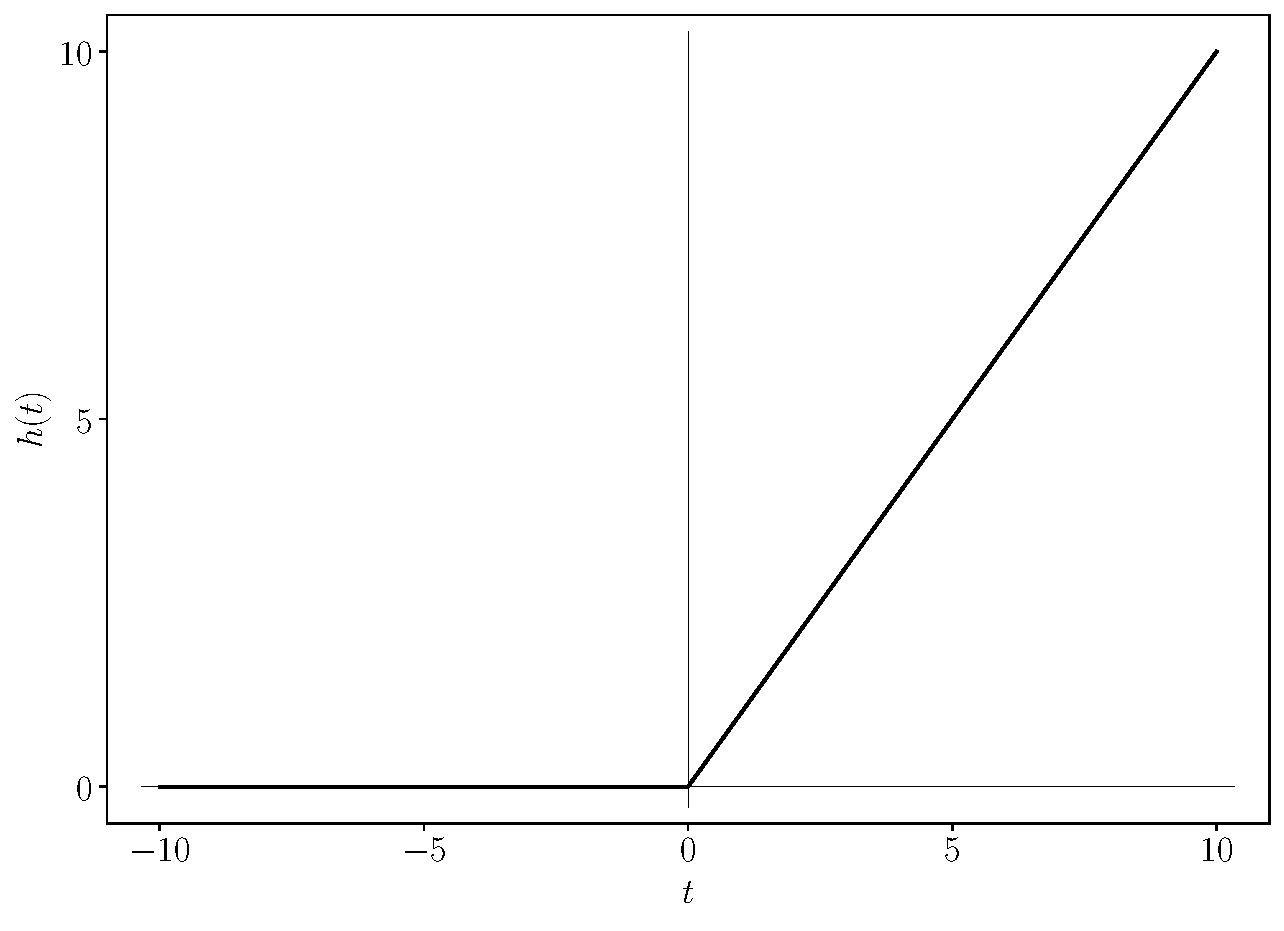
\includegraphics[width=.47\linewidth]{imgs/relu.pdf}
	}
	\subcaptionbox{Leaky \gls{relu} ($\alpha = 0.1$)}{
		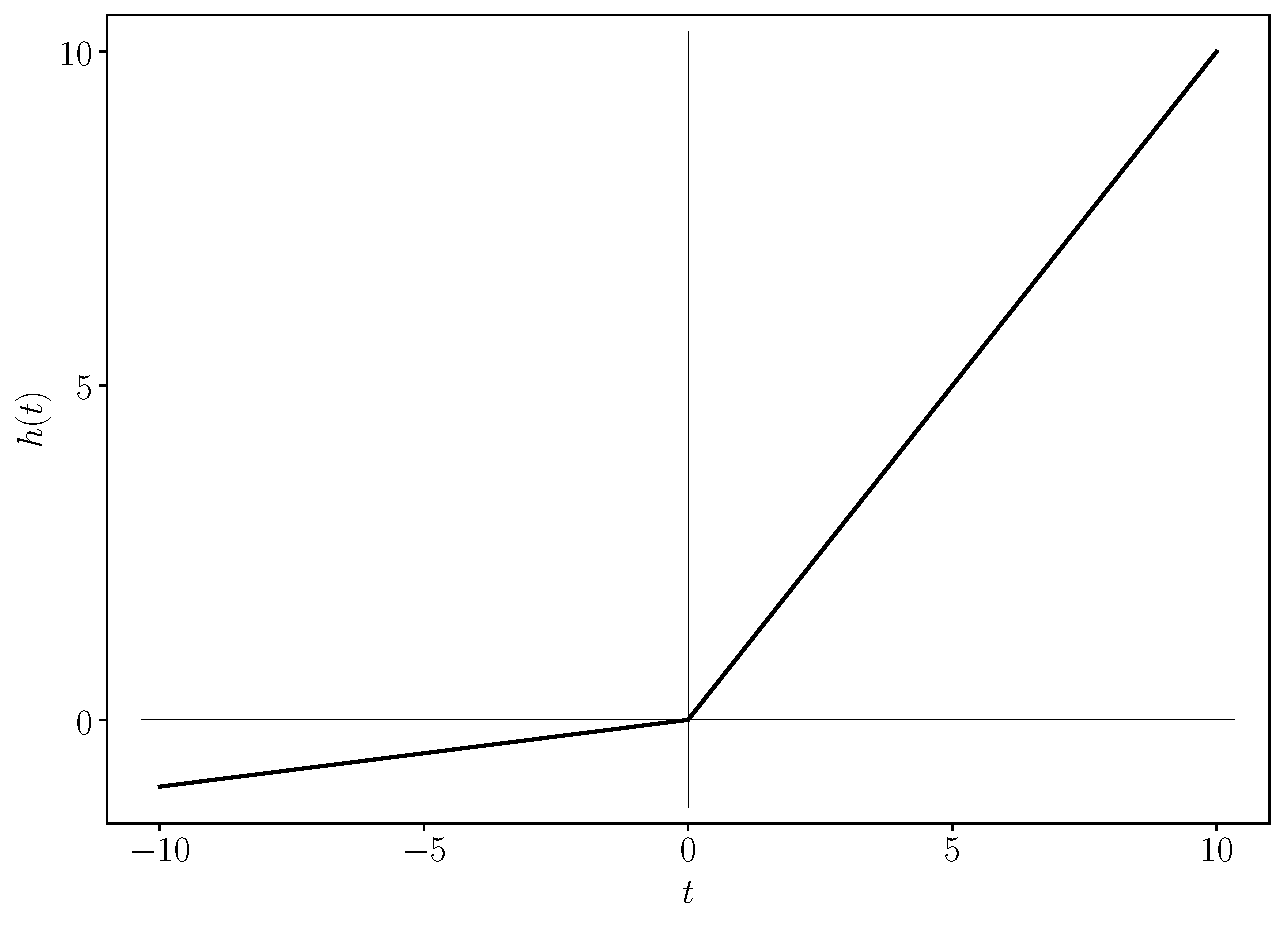
\includegraphics[width=.47\linewidth]{imgs/leaky_relu.pdf}
	}
	\caption{Commonly used activation functions for neural networks}
	\label{fig:act_functions}
\end{figure}

\bigskip
Network weights are learned through gradient based methods. In order to do so, a fundamental step is the definition of a \textit{loss} or \textit{cost} function. Loss functions are mathematical functions that map an event or the values of one or more variables to a real number, which intuitively represents a certain cost associated with these values. Therefore, each training of deep neural networks aims at minimizing or maximizing one or more loss functions that depend on the problem, in order to make network weights evolve in the desired directions. 

\medskip
In a multi-class classification scenario, the output of each output neuron is mapped to the posterior probability of the corresponding class. This is usually done through the \textit{softmax} operation. If the $k$\textsuperscript{th} node of the output layer returns the value $y_k$, it is computed as:
\begin{equation*}
	p(c_k|x) = \frac{\exp{(y_k)}}{\sum_{i=0}^n \exp{(y_i)}}
\end{equation*}
which is therefore the probability that observation $x$ belongs to class $k$. This is computed for all classes and $x$ is usually assigned to the class with the highest probability.

\medskip
According to the \textit{backpropagation} algorithm, classification error or loss is estimated at the output layer, considering incorrectly classified examples, and network weights are updated accordingly, from the output to the input layer. This is done by computing the gradient of the loss function and distributing it backwards on the network neurons, by recursively applying the chain rule of calculus\cite{goodfellow2016deep}. A general schema is reported in Figure~\ref{fig:forwardbackward}.

\begin{figure}[ht]
	\centering
	\subcaptionbox{Forward step}{
		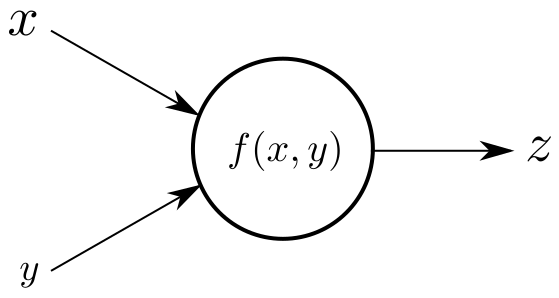
\includegraphics[width=.41\linewidth]{imgs/forward.png}
	}
	\subcaptionbox{Backward step}{
		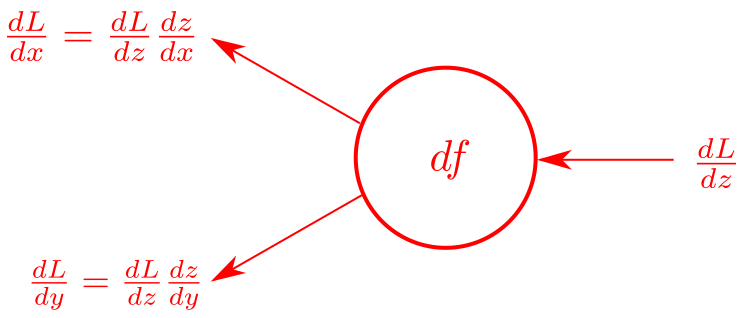
\includegraphics[width=.53\linewidth]{imgs/backward.png}
	}
	\caption{Propagation and backpropagation schema}
	\label{fig:forwardbackward}
\end{figure}

\subsection{Convolutional neural networks}
\Acrfullpl{cnn} are a special class of feedworward neural networks, designed to work with inputs that are organized as grids. Hidden units are organized into grids as well. Indeed, if image pixels were directly fed to a feedforward neural network, the model could not extract meaningful relations between adjacent pixels, possibly taking into account the different color channels.

\bigskip
\Glspl{cnn} are usually composed of two main sections: the first one deals with feature extraction, while the second addresses classification or regression, depending on the desired task. A simple \gls{cnn} architecture is reported in Figure~\ref{fig:cnn}.

\medskip
For feature extraction, following the same principle of \glspl{mlp}, increasingly complex non-linear relationships between adjacent pixels are extracted from input images, by stacking convolutional layers with non-linear activation functions. Linear mappings from one layer to the next one take the form of convolution operations with three-dimensional convolutional filters of fixed size. \textit{Pooling} layers can then be added in order to reduce the size of the extracted feature maps. The goal of pooling is to replace the output of a convolutional layer with a summary of its local statistics, making it more robust to small differences in the input. Popular pooling operators are \textit{max} and \textit{average} pooling.

Different architectures can be used for this part of the network, which is typically referred to as \textit{backbone}.

\medskip
In the most simple case, extracted features are then forwarded to one or more \textit{fully connected} layers, that can be seen as a standard \gls{mlp} introduced in the previous section. The \gls{mlp} assembles all local information into a global vectorial representation and outputs a prediction for the input image.

However, this part of the network depends on the task of interest and several architectures have been proposed over the years. These architectures can be complex and composed of different units for different sub-tasks. They always rely on the features extracted by the backbone, that are potentially shared among all the components of the architecture, as several high level tasks may need to access the same low level features

\begin{figure}
	\centering
	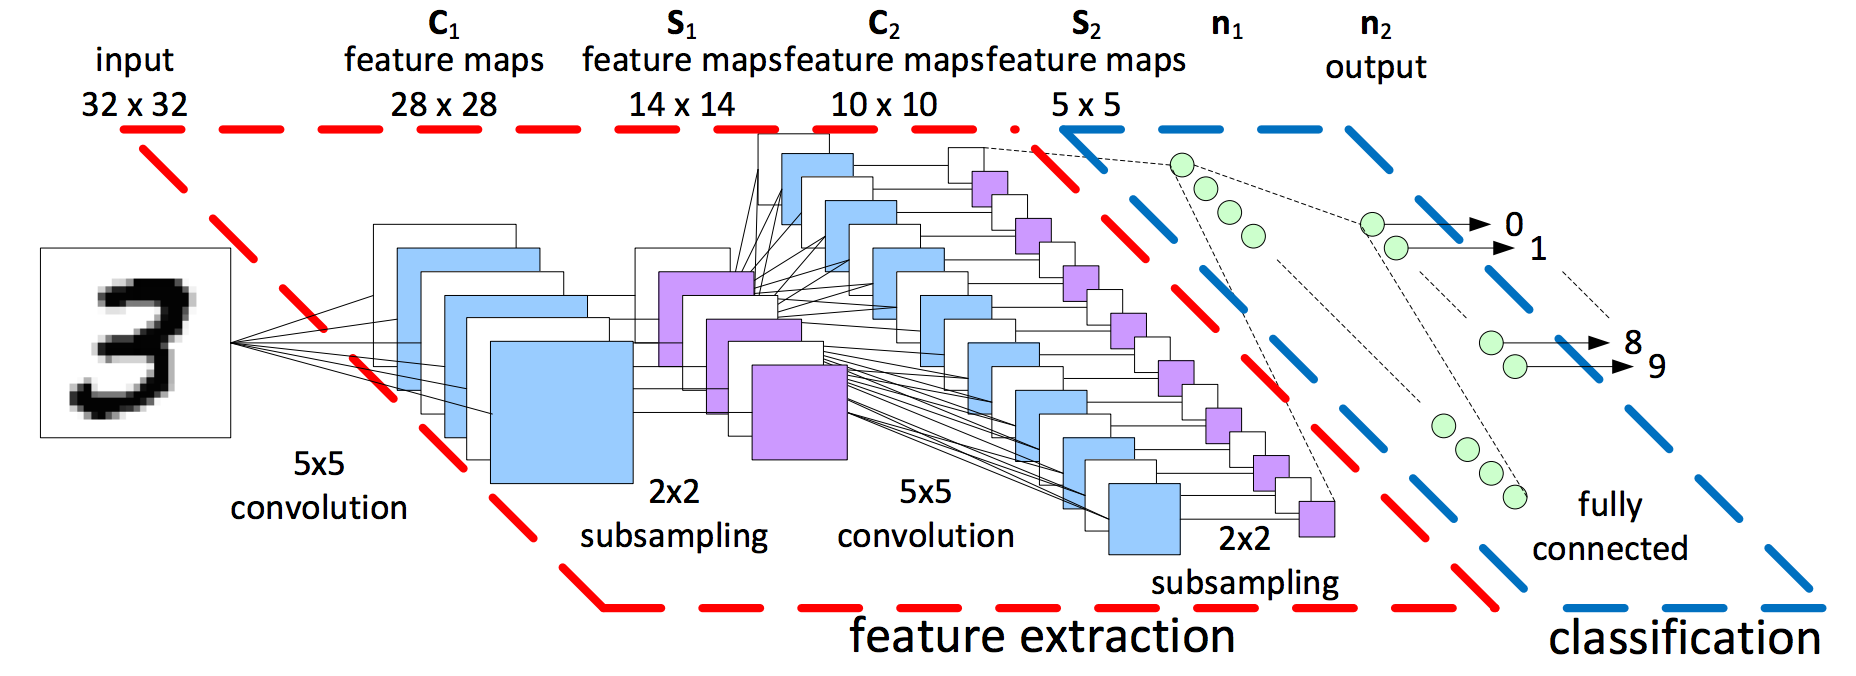
\includegraphics[width=.95\linewidth]{imgs/cnn.png}
	\caption{An example of \gls{cnn} for handwritten digit recognition}
	\label{fig:cnn}
\end{figure}

\subsection{Computer vision}
Before the rise of \glspl{cnn}, computer vision researchers focused on studying effective algorithms to extract information related to the shapes appearing in the images. This is inspired by how animal and human brain works, first focusing on edges or lines, and only after on the full image.

Such algorithms include, but are not limited to, \gls{sift} and \gls{hog}. \Gls{sift} extracts local features from images, with the goal of describing different classes of objects by invariant features\cite{lowe1999object}. \Glspl{hog}, instead, describe images by the number of occurrences of gradient orientations in different portions of the images\cite{dalal2005histograms}. Examples of the algorithms are reported in Figure~\ref{fig:sift_hog}.

\begin{figure}[ht]
	\centering
	\subcaptionbox{\Acrlong{sift}\cite{lowe1999object}}{
		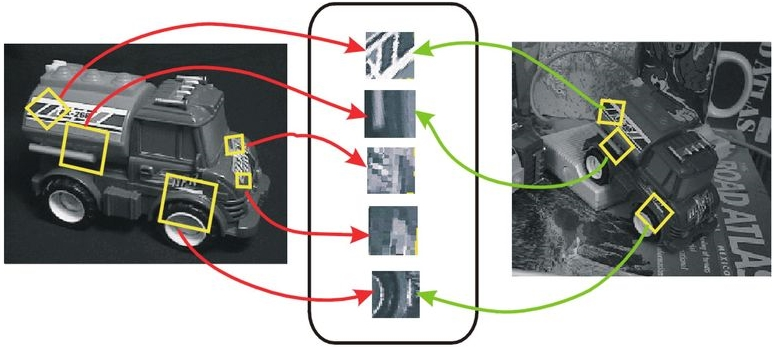
\includegraphics[width=.58\linewidth]{imgs/sift.jpg}
	}
	\subcaptionbox{\Acrlong{hog}\cite{dalal2005histograms}}{
		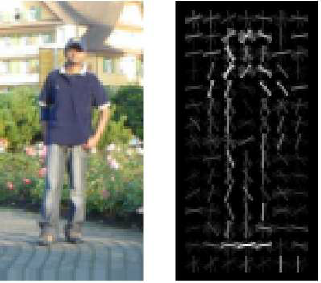
\includegraphics[width=.36\linewidth]{imgs/hog.png}
	}
	\caption{Examples of hand-crafted feature extraction methods}
	\label{fig:sift_hog}
\end{figure}

As mentioned in previous sections, features extracted from available images are then used to train supervised or unsupervised machine learning algorithms, depending on the task of interest.

\medskip
In recent years, \gls{cnn}-based methods have outperformed previous approaches based on manually extracted features and classical machine learning algorithms, since they are able to learn complex relationships in the data by progressively extracting higher-level features from the raw data.
Figure~\ref{fig:imagenet} shows an example of the progresses made by \glspl{cnn} in computer vision.

\begin{figure}[ht]
	\centering
	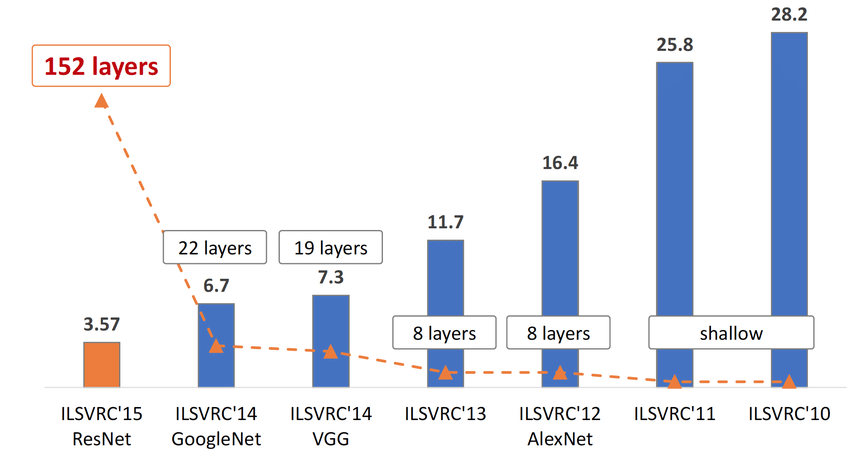
\includegraphics[width=.8\textwidth]{imgs/ILSVRC.png}
	\caption[Evolution of top-5 error for the winning entries in \gls{ilsvrc}]{Evolution over the years of the top-5 error for the winning entries in the \gls{ilsvrc}, from right to left\cite{russakovsky2015imagenet}\cite{hanqing2020research}.
	\label{fig:imagenet}}
\end{figure}

\bigskip
Three main tasks can be identified in computer vision, all of which have benefited from the development of deep convolutional neural network architectures:

\begin{itemize}
	\item \textbf{Image classification}, whose objective is to predict the class label for an image.
	\item \textbf{Object detection}, whose objective is to predict the position and the class label for all the objects that appear in an image, which may belong to different classes. The position of an object is represented by means of rectangular coordinates, called bounding box.
	\item \textbf{Semantic segmentation}, whose objective is to predict a class label for each pixel in an image. A possible extension is \textit{instance segmentation}, which identifies the object instance for each pixel, distinguishing different objects belonging to the same class.
\end{itemize}

A summary is presented in Figure~\ref{fig:classdetseg}.

\begin{figure}
	\centering
	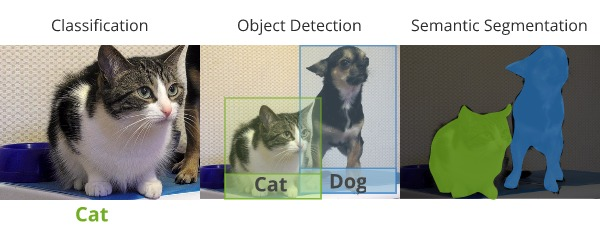
\includegraphics[width=.9\textwidth]{imgs/classification_detection_segmentaion.jpeg}
	\caption[Comparison between classification, object detection and semantic segmentation]{Comparison between classification, object detection and semantic segmentation}
	\label{fig:classdetseg}
\end{figure}

\section{Object detection}\label{sec:detection}
Object detection methods are able to recognize the objects represented in an image and to highlight their position, returning the associated bounding boxes, rectangular boxes which contain an object. The bounding box format depends on the model and on the dataset. Typically, they are determined by the \textit{x} and \textit{y} coordinates of the upper-left corner
%, as in \acrshort{coco} (\ref{sec:coco}),
or of the center
%, as in \acrshort{yolo} (\ref{sec:yolo}),
and by the width and height of the bounding box.

\begin{figure}[ht]
	\centering
	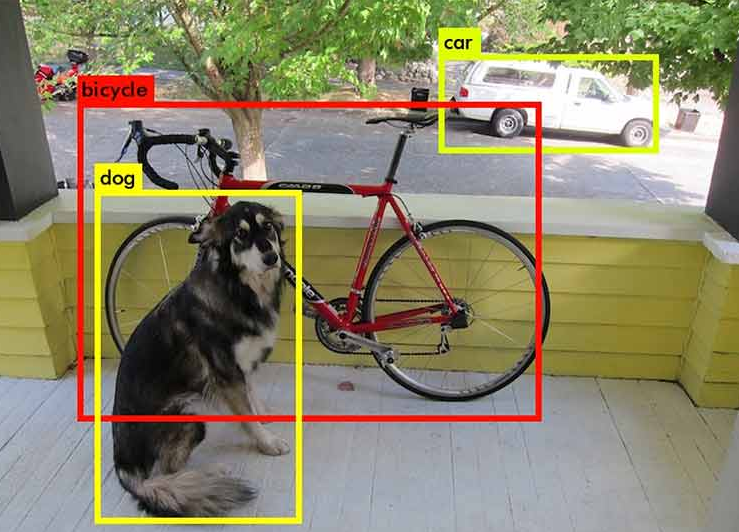
\includegraphics[width=.65\textwidth]{imgs/yolo_detection.png}
	\caption{An example of object detection\cite{redmon2016look}}
\end{figure}

Object detection is a fundamental task in modern computer vision, with applications such as autonomous driving, robot vision and human-computer interaction.

\subsection{Existing methods}\label{sec:detectors}
An object detection task can be seen as a combination of two main steps: finding image regions that may contain objects, and then independently classifying the objects in those regions. Before deep learning, this was achieved using a sliding-window approach, where an image classifier was applied to different areas of the image and only the predictions with the highest probability were retained. Nowadays, two main families of object detectors can be identified.

\bigskip
Several network architectures have been using as backbones of object detectors, to extract features from input images to be fed to the high-level network components for the object detection task. Due to high performances, one of the most popular choices is exploiting a \gls{resnet} architecture\cite{he2015deep}.

\Glspl{resnet} are neural networks characterized by the use of \textit{shortcuts} or \textit{skip connections}. Through these skip connections, the output of a network block is added to the same signal it received as input. This favors the transmission of the gradient from high level to low level layers during the backpropagation phase, avoiding \textit{vanishing gradient}. The contribution of the information extracted by the first network layers during inference is favored as well. This has allowed the implementation of very deep networks, solving the problems encountered by previous architectures concerning training and accuracy. The structure of a residual block is reported in Figure~\ref{fig:resnet}.

The number of layers of a \gls{resnet} is usually specified as a suffix. Common values are 18, 34, 50 (\gls{resnet}-50), 152, up to over 1000 layers\cite{he2016identity}.

\begin{figure}[ht]
	\centering
	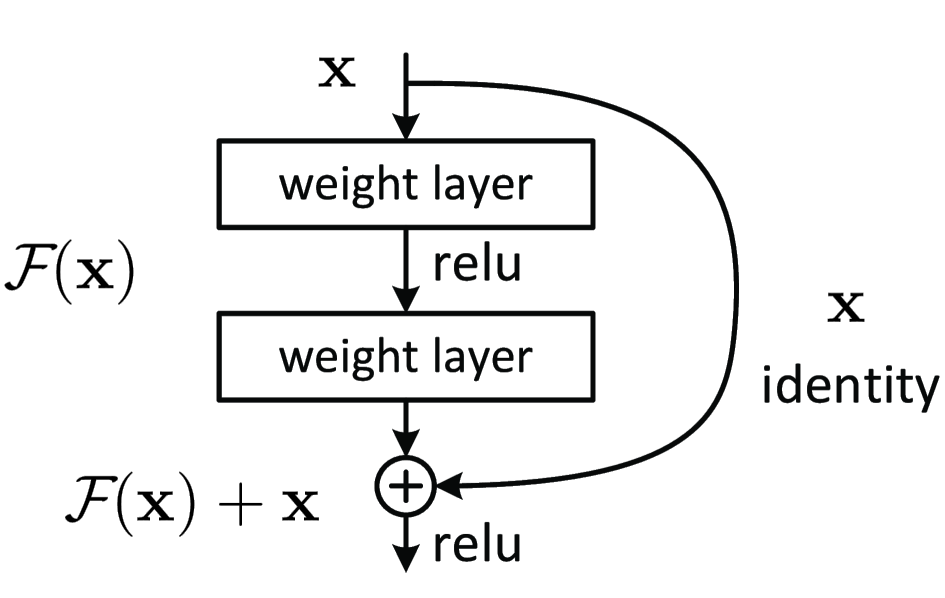
\includegraphics[width=.5\textwidth]{imgs/resnet.png}
	\caption{An example of building block for residual learning\cite{he2015deep}}
	\label{fig:resnet}
\end{figure}

\subsubsection{Two stage object detectors}
As said, the most commonly used models for object detection are based on a two-stage approach and belong to the family of \glspl{rcnn}. In basic \gls{rcnn}\cite{girshick2014rich}, a manageable number of possible \glspl{roi} are extracted from an image, following the \textit{Selective Search} algorithm.

Selective search aims at localizing objects in the input images, and is pitted against previously used \textit{Exhaustive Search}, in which the sliding-window approach is followed to detect \glspl{roi}. In selective search, an input image is initially segmented in small regions, which are then recursively merged according to their similarity. The operation is repeated until bigger independent regions are generated. These regions are returned as candidate \glspl{roi}.

A \gls{cnn} is then evaluated independently on each proposed \gls{roi} to extract features that are fed into a \gls{svm}
%to classify the presence of an object in that region and the bounding box location.
to determine if an object is present in this bounding box (classification task) as well as its location to match that of the object (regression task). As \gls{svm} is a binary classification algorithm, as many \glspl{svm} as classes of interest are used for the classification task. A summary of the method is reported in Figure~\ref{fig:rcnn}.

\begin{figure}[ht]
	\centering
	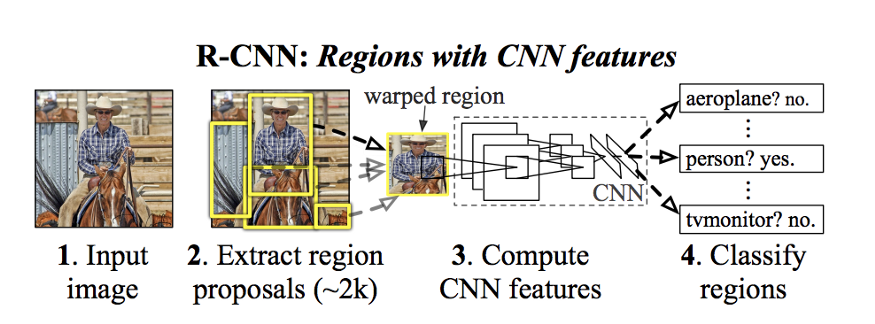
\includegraphics[width=.8\linewidth]{imgs/rcnn.png}
	\caption{Description of standard \gls{rcnn}\cite{girshick2014rich}}
	\label{fig:rcnn}
\end{figure}

\medskip
Fast \gls{rcnn}\cite{girshick2015fast} and Faster \gls{rcnn}\cite{ren2016faster} enhanced the \gls{rcnn} architecture, improving its performances and reducing the inference time.

\paragraph{Fast \gls{rcnn}}
In Fast \gls{rcnn}\cite{girshick2015fast}, performances are improved through the introduction of a \textit{\gls{roi} pooling} layer and of a single-stage training procedure with an optimized multi-task loss.

\medskip
\Gls{roi} pooling layer allowed to solve one of the main sources of slowness of the previous \gls{rcnn} architecture: as described, in \gls{rcnn} each proposed \gls{roi} is independently fed to a \gls{cnn} for feature extraction.

With \gls{roi} pooling, the whole input image is forwarded only once to the feature extractor. Rectangular feature maps, corresponding to each proposed \gls{roi}, are then extracted from the image's features.

\medskip
Following a single-stage training, instead, Fast \gls{rcnn} discards the previously used \glspl{svm} for classification. Two sibling output layers are used:
\begin{itemize}
	\item the classification head returns, through softmax and for each \gls{roi}, a discrete probability distribution $p$ over $K+1$ categories (the $K$ classes of interest and an \quotes{extra} background class);
	\item the regression head returns, for each \gls{roi} and class $k$, a bounding box offset $t^k$, which specifies a scale invariant translation and height/width shift in logarithmic space.
\end{itemize}

The two heads are trained jointly, thanks to a purpose-built loss function that takes into consideration both classification and regression tasks. For each couple of classes $u, v$, with $u$ ground truth class, this multi-task loss is defined as:
\begin{equation}
	L(p,u,t^u,v) = L_{\text{cls}}(p,u) + \lambda\left[u\geq1\right]L_{\text{loc}}(t^u,v).
	\label{eq:fastrcnn}
\end{equation}

Here, $L_{\text{cls}}(p,u) = -\log{p_u}$ is the standard negative log-likelihood for the correct class $u$ and is responsible for the training the classification head. $L_{\text{loc}}(t^u,v)$ is instead responsible for the regression head and is defined as a robust $L_1$ loss:
\begin{equation*}
	L_{\text{loc}}(t^u,v) = \sum_{i\in \text{\{x,y,w,h\}}}\text{smooth}_{L_1}(t_i^u - v_i)
\end{equation*}
in which
\begin{equation*}
	\text{smooth}_{L_1}(x) = \begin{cases}
		0.5x^2 & \text{if } |x| < 1\\
		|x| - 0.5 & \text{otherwise.}
		\end{cases}
\end{equation*}

$\left[u\geq1\right]$ is an indicator function that evaluates to $1$ when $u\geq1$ and $0$ otherwise, meaning that the regression head is not trained for \glspl{roi} belonging to the background class (labeled $u=0$ by convention). Indeed, the concept of ground truth bounding boxes does not make sense for background regions.

Finally, the $\lambda$ hyperparameter is used to assign a relative weight to the two tasks.

\paragraph{Faster \gls{rcnn}}\label{sec:fasterrcnn}
The main contribution of Faster \gls{rcnn}\cite{ren2016faster} over Fast \gls{rcnn} is the introduction of a \gls{rpn}, which integrates some convolutional layers of the image classifier into the region proposal phase. It is designed to replace selective search, an expensive and time-consuming algorithm, and helps to considerably reduce the required time. Faster \gls{rcnn} working scheme is reported in Figure~\ref{fig:fasterrcnn}.

\begin{figure}[ht]
	\centering
	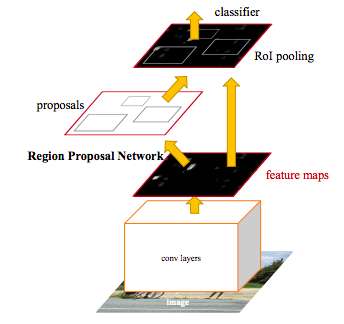
\includegraphics[width=.5\linewidth]{imgs/fasterrcnn.png}
	\caption{Description of Faster \gls{rcnn}\cite{ren2016faster}}
	\label{fig:fasterrcnn}
\end{figure}

\medskip
The goal of \gls{rpn} is to extract a set of \glspl{roi} from an input image, each with a probability that it contains indeed an object instead of a background region. Basically, this \gls{cnn} shares a common set of convolutional layers with a Fast \gls{rcnn} object detector and highlights the image regions on which it should focus.

In order to generate \gls{roi} proposals, the \gls{rpn} receives as input the features extracted by the last shared convolutional layer, and a sliding-window approach is followed to extract multiple proposals. Each \gls{roi} is mapped to a lower-dimensional feature map, which is fed to two sibling fully-connected layers: a binary classification layer which estimates the probability that the input \gls{roi} actually contains an object, and a box-regression layer to refine the bounding box proposals.

The regions that are generated at each sliding-window location have different sizes and aspect rations and are called \textit{anchor boxes}. This is an important concept in modern object detection, and is further detailed in Section~\ref{sec:anchor}.

\Gls{rpn} can then be trained with the goal of minimizing a multi-task loss function that follows the same reasoning of \eqref{eq:fastrcnn}.

\medskip
However, the \gls{rpn} and the Fast \gls{rcnn} detector share a set of convolutional layers: independent training of the two components would modify the weights in different ways and results would be inconsistent. Three techniques are proposed for jointly training networks with shared features:
\begin{itemize}
	\item \textit{Alternating training}: the \gls{rpn} is initialized as a pre-trained \gls{cnn} and fine-tuned end-to-end on the \gls{roi} proposal task, and the generated proposals are used to train a Fast \gls{rcnn} object detection network. In this phase, no convolutional layer is shared among the two networks. Fast \gls{rcnn} is then used to initialize \gls{rpn} training, but fixing shared layers and fine-tuning only the ones unique to \gls{rpn}, making the two components share convolutional layers. Finally, shared layers are kept fixed and unique layers of Fast \gls{rcnn} are fine-tuned. The process can be repeated for many iterations.
	\item \textit{Approximate joint training}: \gls{rpn} and Fast \gls{rcnn} components are merged into one network. However, this joint training leads to approximate results, as \gls{roi} proposals are treated like fixed, pre-computed proposals when training the Fast \gls{rcnn}. For this reason, during backpropagation the fact that the proposed bounding boxes' coordinates depend on the \gls{rpn} is ignored.
	\item \textit{Non-approximate joint training}: the above-mentioned problem could be resolved by computing gradients with respect to the box coordinates in the backpropagation step. This would require the development of a \gls{roi} pooling layer that is differentiable with respect to box coordinates. This is a nontrivial problem.
\end{itemize}

\medskip
Because of its good performances and speed, Faster \gls{rcnn} is widely used for benchmarking and as base for several derived works.

\subsubsection{One stage object detectors}
Differently from two stage detectors, one stage object detectors skip the region proposal phase and focus on predicting object regions and classes together. This leads to faster predictions with respect to two stage models, making them suitable for real-time applications at the cost of lower prediction quality. The pioneer work for one stage object detection is OverFeat\cite{sermanet2014overfeat}, published in 2014. Here, the last classification layers of a standard \gls{cnn} are replaced by a regression network for each class, in order to predict the coordinates of the object bounding boxes.

\paragraph{YOLO}\label{sec:yolo}
The \gls{yolo} model\cite{redmon2016look} uses pretrained \gls{cnn} for classification and splits each image in cells. If the center of an object falls into a cell, that cell is responsible for detection and should predict the bounding box locations, a confidence score and a class probability for the detected objects. A specific loss function is used to efficiently learn to predict bounding boxes and object classes at the same time.

\paragraph{SSD}
\gls{ssd}\cite{Liu_2016} uses a VGG-16 convolutional network as backbone and adds on top several convolutional layers of decreasing sizes, in order to build a \textit{pyramid representation} of the images and efficiently detect object of different sizes, at each pyramid layer. Instead of splitting images in cells, anchor boxes are used for faster detection.

\begin{figure}[ht]
	\centering
	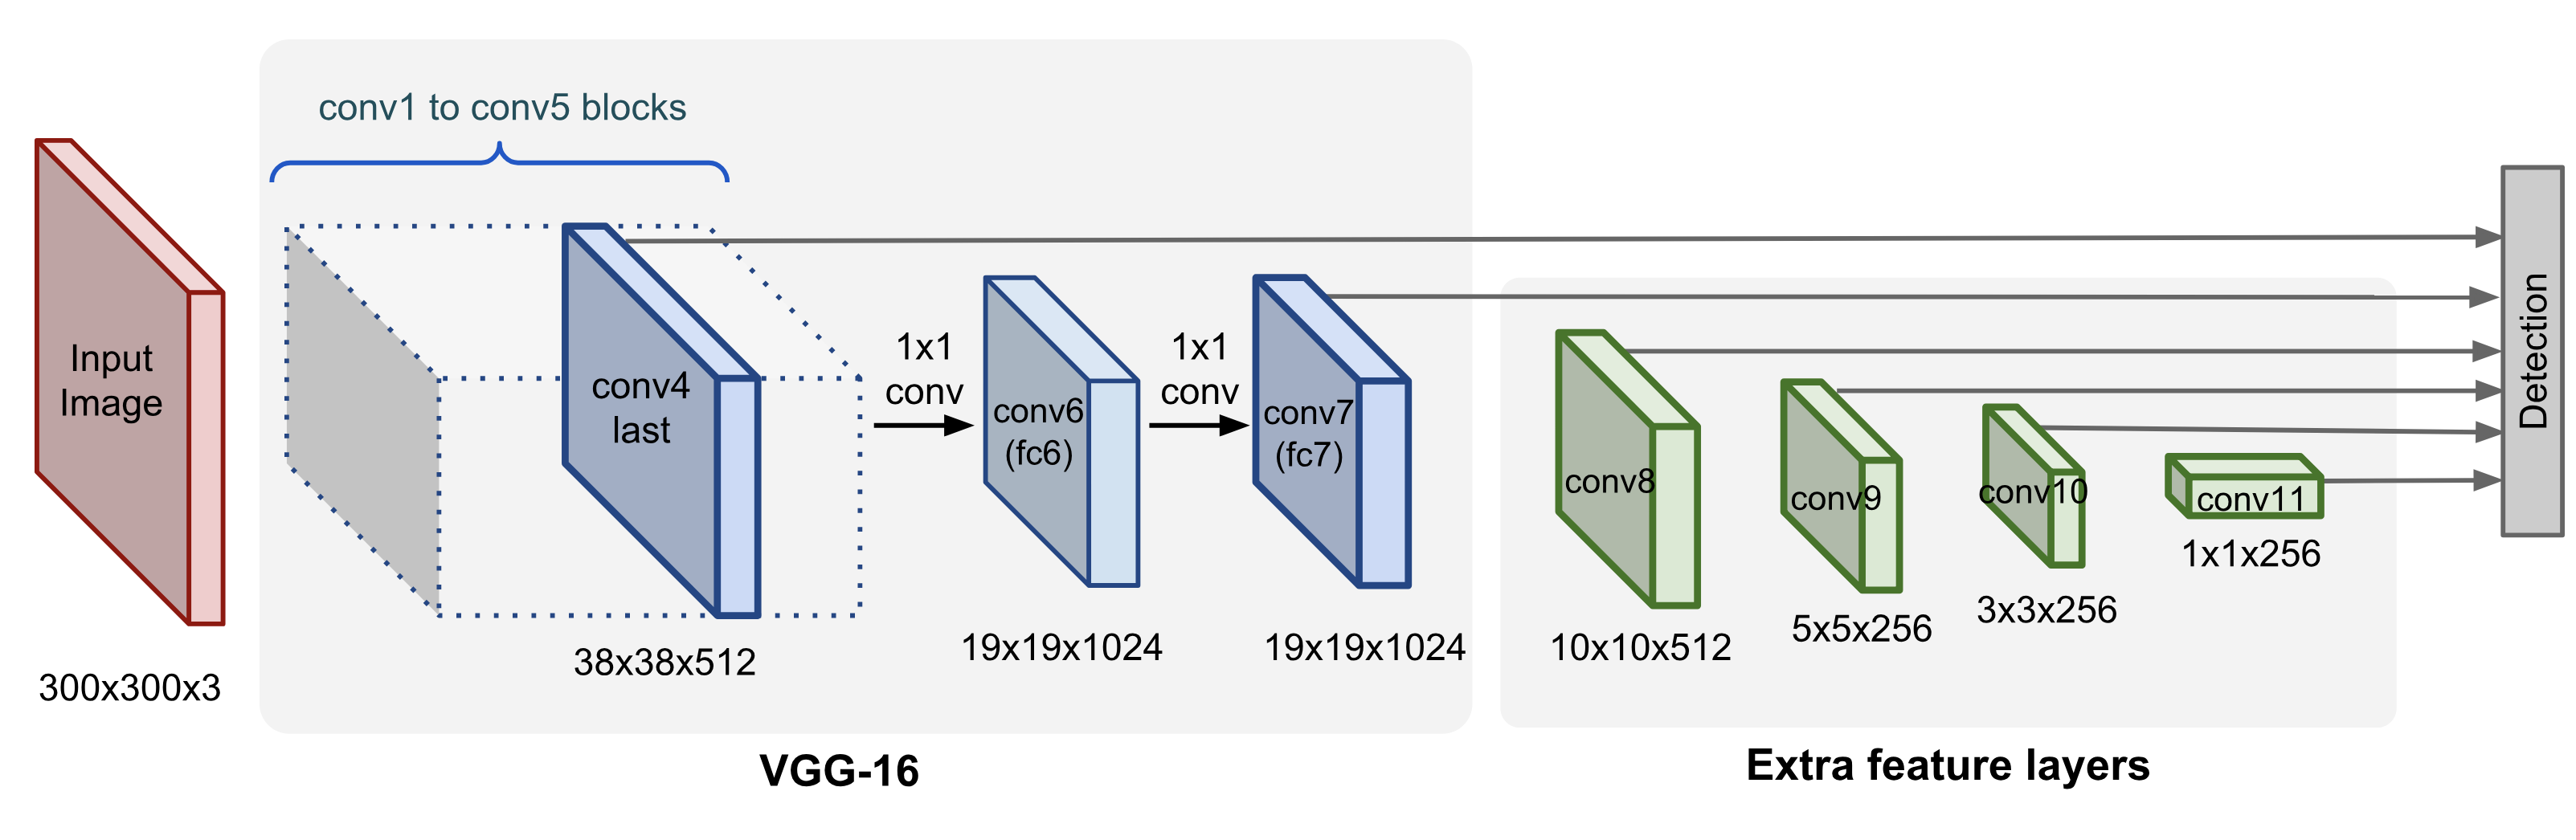
\includegraphics[width=.9\linewidth]{imgs/SSD-architecture.png}
	\caption{\acrshort{ssd}'s pyramid architecture\cite{objdetpart4}}
	\label{fig:ssd}
\end{figure}

After their proposal, \gls{yolo} and \gls{ssd} have both been extensively studied and improved by the research community. The last versions of the two families are architecturally close and work in very similar ways.

\paragraph{RetinaNet}
The main improvements of RetinaNet\cite{lin2018focal} over previous one stage detection models are the use of \gls{fpn} as part of the backbone and of \textit{focal loss}, which helps to approach the results of two-stage detectors.

\begin{figure}[b]
	\centering
	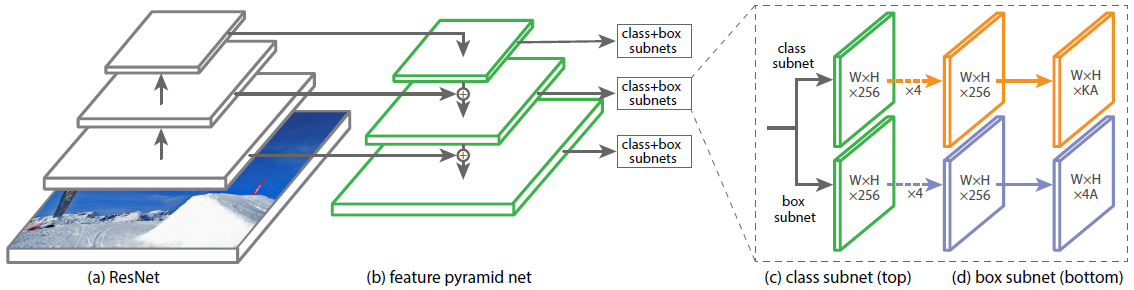
\includegraphics[width=\linewidth]{imgs/retinanet.png}
	\caption{RetinaNet architecture\cite{lin2018focal}}
	\label{fig:retinanet}
\end{figure}

\subparagraph{Feature Pyramid Network}
\glspl{fpn}\cite{lin2017feature} adopt and improve the same approach as \acrshort{ssd}'s pyramid layers. They are built of a sequence of pyramid levels which correspond to network stages. Each stage is composed by multiple convolutional layers of the same size, divided by two at consecutive stages. In addition to standard feedforward, different stages are linked by a top-down pathway in the opposite direction, together with lateral connections. This allows the network to construct a rich and multiscale feature pyramid for each input image.

After their proposal in the context of single-stage detectors, \glspl{fpn} have also been used as part of the backbone of two-stage detectors, aiming at improving their performances.

\subparagraph{Focal loss}
One of the main obstacles for the training of other object detection models is the large imbalance between background and foreground examples, which drives the model to focus on irrelevant background regions.
%Loss functions are one of the fundamental bricks of deep learning: they are mathematical functions that map an event or the values of one or more variables to a real number, which intuitively represents a certain cost associated with these values. Therefore, each training of deep neural networks aims at minimizing or maximizing one or more loss functions that depend on the problem.
As explained in previous sections, each training of deep neural networks aims at minimizing or maximizing one or more loss functions that depend on the problem.
In this case, a specific loss function can be used to encourage the network to focus on regions of the images that actually contain objects.

\bigskip
The \textit{focal loss}, introduced by RetinaNet, is based on the \textit{cross entropy} loss. For binary classification, the cross entropy loss is widely used and defined as:
\begin{equation}
	\text{CE}(p,y) = \begin{cases}
		-\log(p) & \text{if $y$ = 1}\\
		-\log(1-p) & \text{otherwise}
	\end{cases}
\end{equation}
where $y\in \{\pm 1\}$ is the ground truth class and $p\in\left[0,1\right]$ is the model's probability for class $1$. In this context, $y=1$ and $y=-1$ represent the foreground and background classes respectively. Defining $p_t$ as:
\begin{equation}
	p_t = \begin{cases}
		p & \text{if $y$ = 1}\\
		1-p & \text{otherwise}
	\end{cases}
\end{equation}
cross entropy can be written as $\text{CE}(p,y) = \text{CE}(p_t) = -\log(p_t)$.

\bigskip
A balanced version of the cross entropy loss is sometimes used to deal with class imbalance. A numeric factor $\alpha\in\left[0,1\right]$ can be introduced for class $1$, with value $1-\alpha$ for class $-1$. $\alpha_t$ is defined analogously to $p_t$. Therefore, the cross entropy loss, balanced by $\alpha_t$, is written as:
\begin{equation}
	\text{CE}(p,y) = -\alpha_t\log(p_t).
\end{equation}

\bigskip
With cross entropy, also examples that are correctly classified with high confidence ($p$ close to $1$ if $y=1$, to $0$ otherwise) produce non-negligible values for the loss.

In focal loss, an additional modulating factor $\left(1-p_t\right)^\gamma$ is introduced, with tunable focusing parameter $\gamma$. Focal loss is therefore defined as:
\begin{equation}
	\text{FL}(p_t) = -\left(1-p_t\right)^\gamma \log(p_t)
\end{equation}
The contribution of easy predictions to the overall loss is more or less important depending on the value of $\gamma$. With a high $\gamma$, well detected objects provide a very little contribution to the total loss.

Considering the strong imbalance between the foreground ($y=1$) and background ($y=-1$) classes, the focal loss balanced by the $\alpha_t$ parameter as previously defined is used in RetinaNet:
\begin{equation}
	\text{FL}(p_t) = -\alpha_t\left(1-p_t\right)^\gamma \log(p_t).
	\label{eq:focalloss}
\end{equation}

\subsection{Basic components}

This section introduces some basic aspects of object detection models. They are necessary to understand the following sections and the performed work.

\subsubsection{Object detection metrics}
Algorithm evaluation is a fundamental part of machine learning projects and can be performed in different ways, depending on the task and objective. Object detection is a more complex task than traditional image classification: a non-fixed number of objects can be present in the same image and the detection model has to accurately predict their class, together with their position. For this reason, dedicated metrics must be introduced and defined.

\paragraph{Precision and recall}
First, the following concepts must be defined in the context of object detection:
\begin{itemize}
	\item \textbf{True positive} (TP): a bounding box is correctly assigned to an object that actually appears in the image;
	\item \textbf{False positive} (FP): incorrect detection, an object is detected but is not really present in the bounding box or only partly;
	\item \textbf{False negative} (FN): an object present is the image is not detected by the object detection model.
\end{itemize}
The concept of true negative (TN) does not make sense in an object detection context, as the missing detection of a non-present object is not relevant. In fact, this would mean that the model has correctly identified the background as not belonging to any class.

\subparagraph{Precision}
Precision measures how accurate the predictions of the model are, so it returns the percentage or fraction of correct predictions.
\begin{equation}
	\text{precision} = \frac{\text{TP}}{\text{TP}+\text{FP}}
\end{equation}

\subparagraph{Recall}
Recall measures the model detection ability, so it returns the percentage or fraction of correctly detected objects.
\begin{equation}
	\text{recall} = \frac{\text{TP}}{\text{TP}+\text{FN}}
\end{equation}

\paragraph{Intersection over union}
For each predicted bounding box, the overlapping with the ground truth bounding boxes is computed, in order to classify a prediction as true or false positive. For a couple of bounding boxes, \gls{iou} is computed as:
\begin{equation}
	\text{IoU} = \frac{\text{area of overlap}}{\text{area of union}}
\end{equation}

The resulting value is then compared to a threshold to classify a prediction as correct or not. Typical values for the threshold are $0.5$, $0.75$ and $0.95$, and that defines how much we want a detection to be precise. Indeed, a prediction classified as true positive with a certain threshold may be considered as false positive if a higher value is used.

\begin{figure}[t]
	\centering
	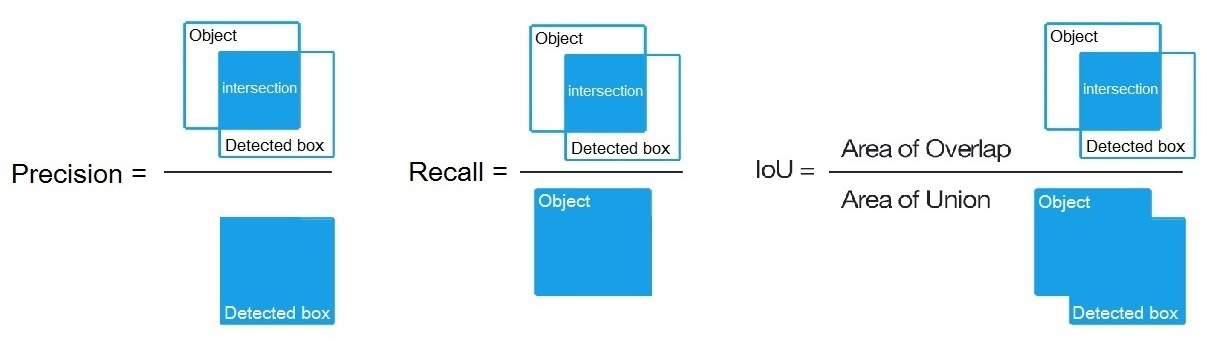
\includegraphics[width=\linewidth]{imgs/precision_recall_iou.jpg}
	\caption[Graphical representations of precision, recall and \gls{iou}]{Graphical representations of precision, recall and \gls{iou}}
	\label{fig:iou}
\end{figure}

\paragraph{Mean Average Precision (mAP)}
\gls{roc} curve is a popular concept in machine learning. There, recall (the true positive rate) and false positive rate are plotted at different classification thresholds. The associated \gls{auc} metric considers the area under the \gls{roc} curve to assess the performances of a model\cite{roc}. It ranges from $ 0 $ to $ 1 $, with $ 0 $ meaning the model's predictions are all wrong and $ 1 $ they are all correct. \Gls{auc} score is $ 0.5 $ for a model that always returns random predictions.

\medskip
Similarly, the precision-recall curve shows the trade-off between precision and recall for different thresholds\cite{precrecall}. \gls{ap} is defined as the area under the precision-recall curve. A high area under the curve means both high recall and high precision. The definition of \gls{map} depends on the context. If \gls{ap} is independently computed for each class or for different \gls{iou} thresholds, then \gls{map} is the average of \gls{ap}. In other cases, \gls{map} and \gls{ap} can be used interchangeably.

\begin{figure}[ht]
	\centering
	\subcaptionbox{\Gls{roc} curve}{
		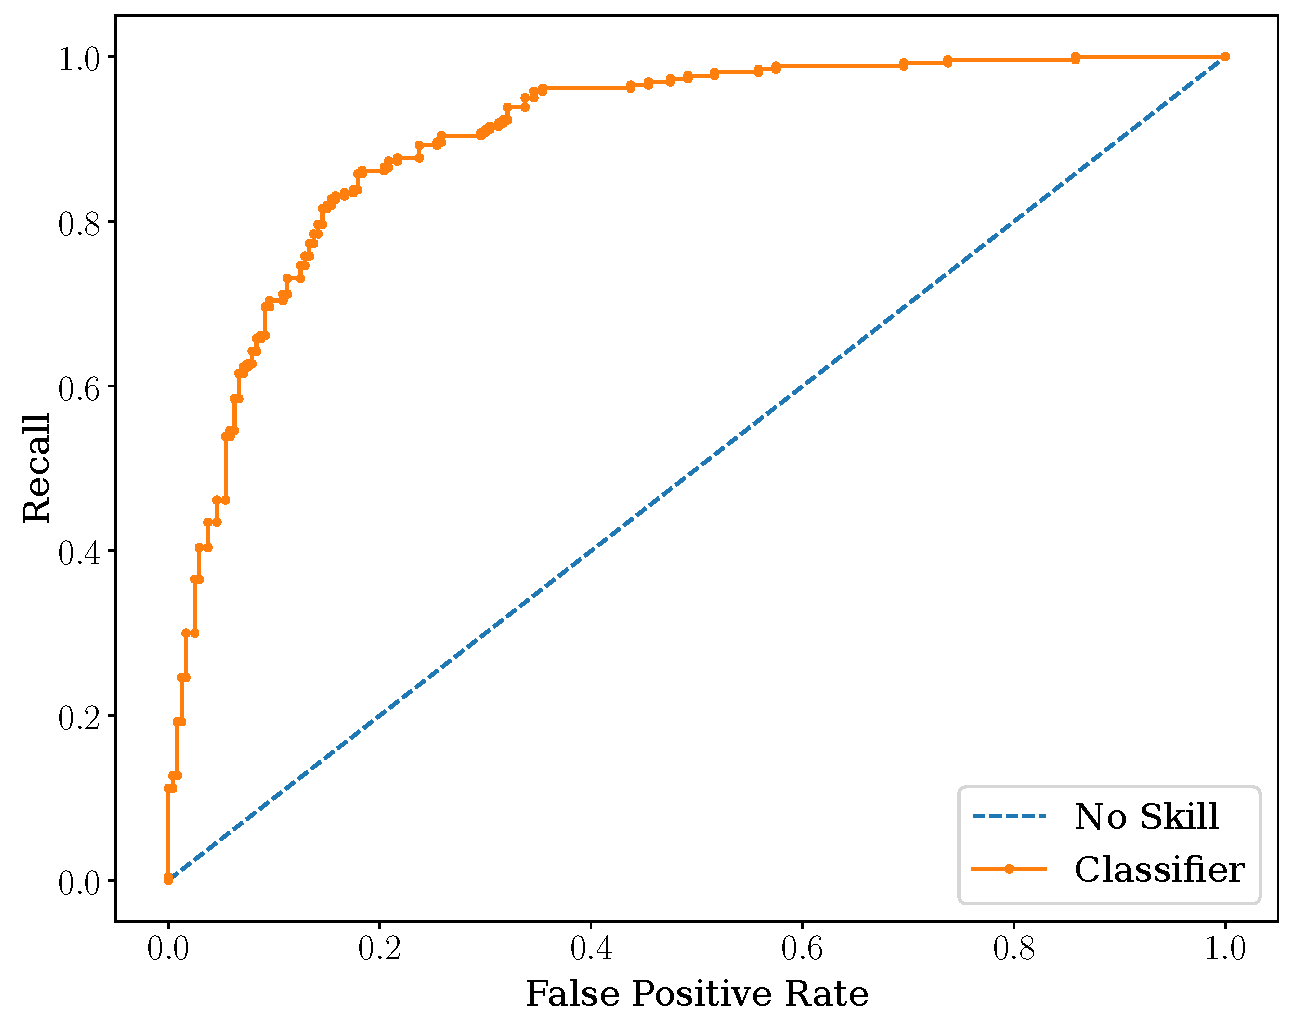
\includegraphics[width=.47\linewidth]{imgs/roc.pdf}
	}
	\subcaptionbox{Precision-recall curve}{
		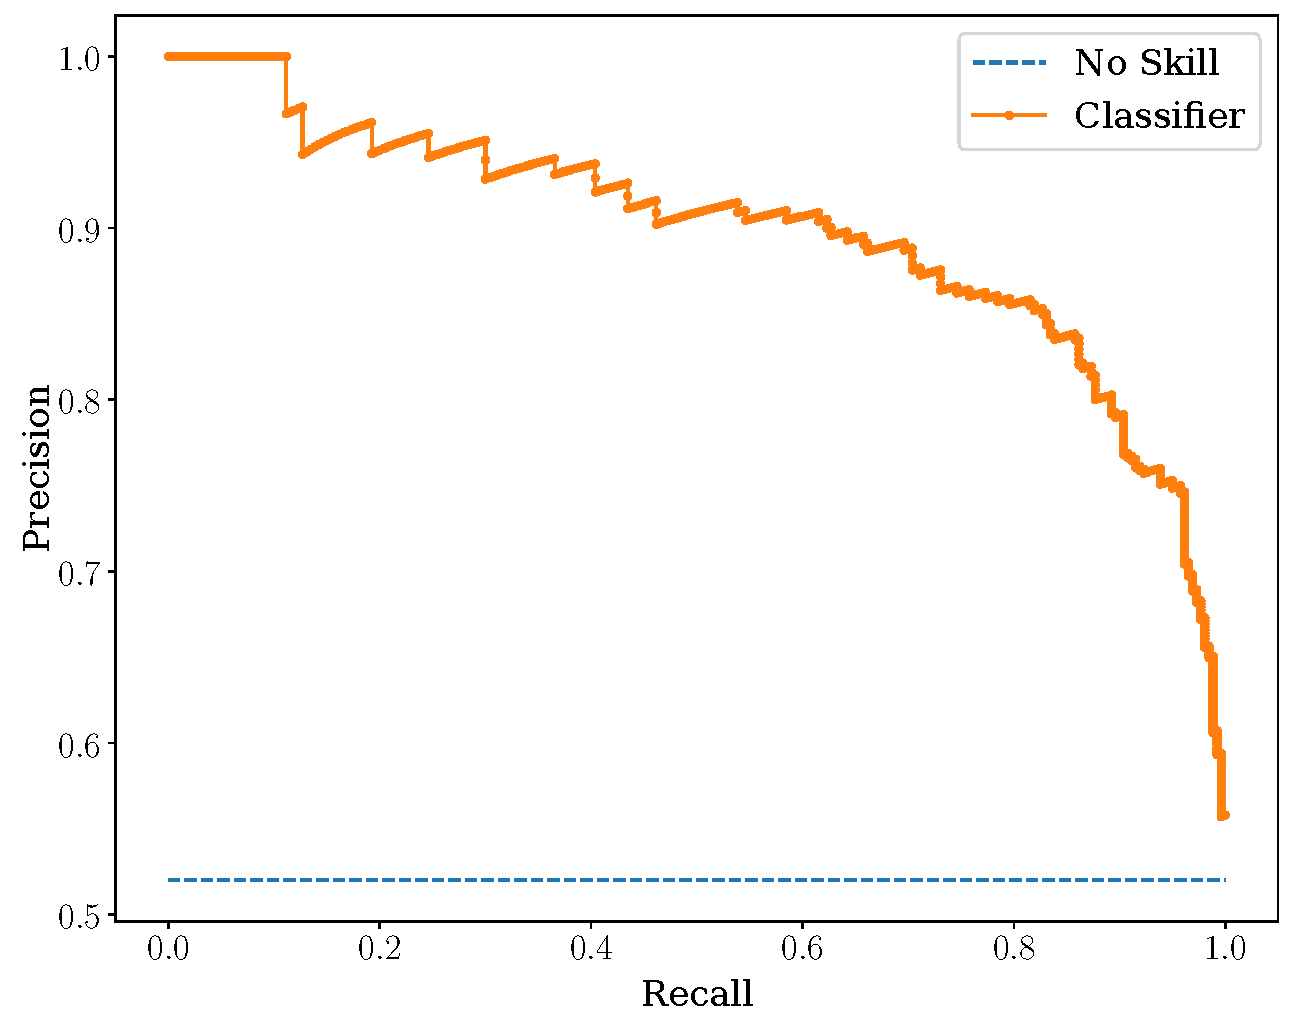
\includegraphics[width=.47\linewidth]{imgs/precision_recall.pdf}
	}
	\caption{Comparison between \gls{roc} curve and precision-recall curve for a trained classifier}
	\label{fig:roc_map}
\end{figure}

\subsubsection{Datasets}\label{sec:datasets}
Several datasets have been published in the last years, with the purpose of training and evaluating the performances of object detection algorithms for different use cases.

\paragraph{COCO}\label{sec:coco}
\gls{coco} is a large-scale object detection and object segmentation dataset published by Microsoft, containing over 200000 images for 91 classes, annotated with bounding boxes and at pixel level\cite{lin2015microsoft}. It defines its own annotation format as \acrshort{json} files.

\paragraph{PASCAL VOC}
PASCAL \gls{voc} is a classification and object detection dataset, developed for different machine learning competitions between 2005 and 2012\cite{voc}. Annotations are stored in \acrshort{xml} format, with a file for each image in the dataset. Bounding boxes are determined by the $x$ and $y$ coordinates of the upper left and bottom right corners.

\paragraph{CityScapes}
CityScapes is an object segmentation dataset containing 5000 street scenes images from 50 different cities, with the aim of training models for autonomous driving\cite{cordts2016cityscapes}. When used for object detection, bounding boxes can be derived from the tightest rectangles containing the segmentation masks.

Several variations of the dataset have been proposed with artificially added adverse weather, such as fog\cite{sakaridis2018semantic} and rain\cite{halder2019physicsbased}, in order to evaluate the robustness of detection methods in various weather conditions.

\paragraph{KITTI}
The \gls{kitti} dataset\cite{Geiger2013IJRR} contains 7481 images captured in a context similar to CityScapes. Bounding box annotations are stored in plain text, with one file per image.

\paragraph{Sim10k}
Sim10k is a synthetic dataset containing 10000 annotated images for car detection, rendered from the popular open-world video-game \textit{Grand Theft Auto 5}, with the objective of training models in a rich virtual world for detection in the real\cite{johnsonroberson2017driving}.

\begin{figure}[p]
	\centering
	\subcaptionbox{CityScapes\cite{cordts2016cityscapes}}{
		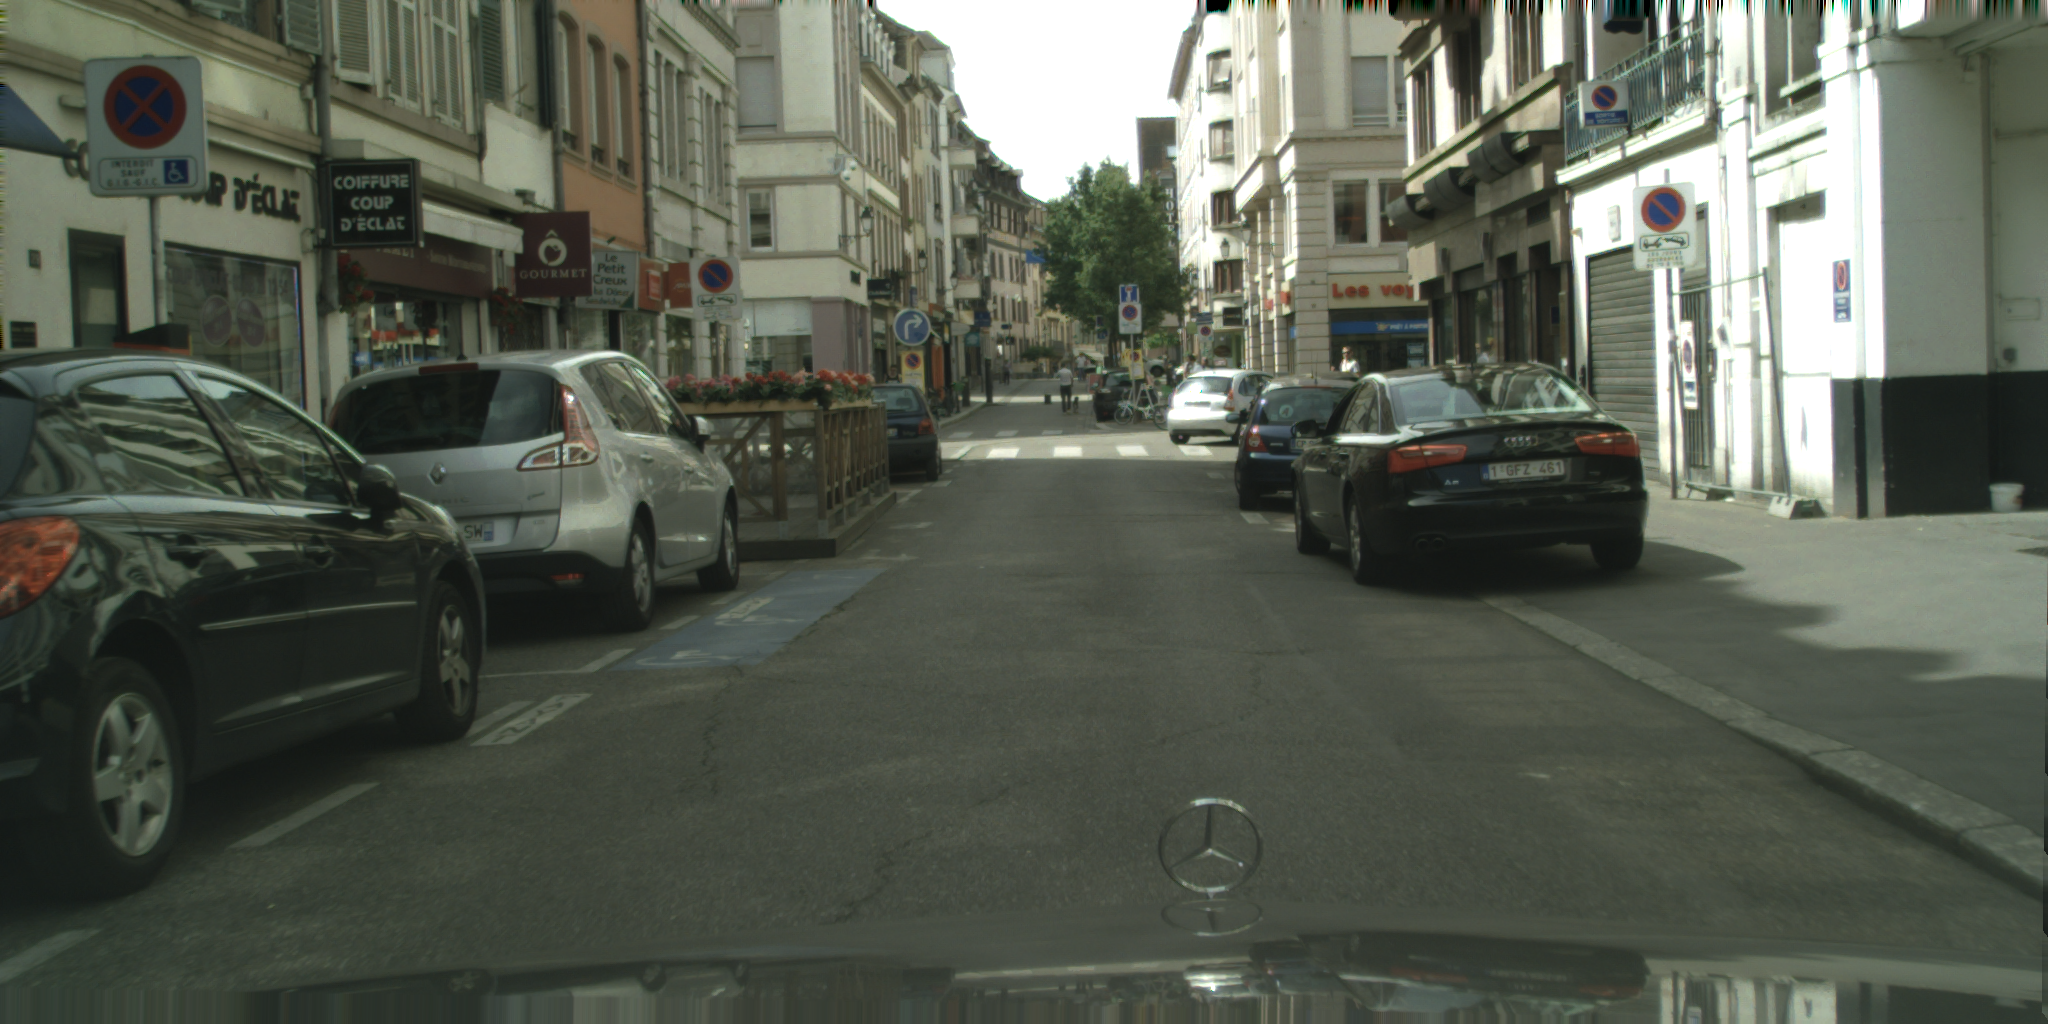
\includegraphics[width=.75\linewidth]{imgs/cityscapes.png}
	}
	\subcaptionbox{\acrshort{kitti}\cite{Geiger2013IJRR}}{
		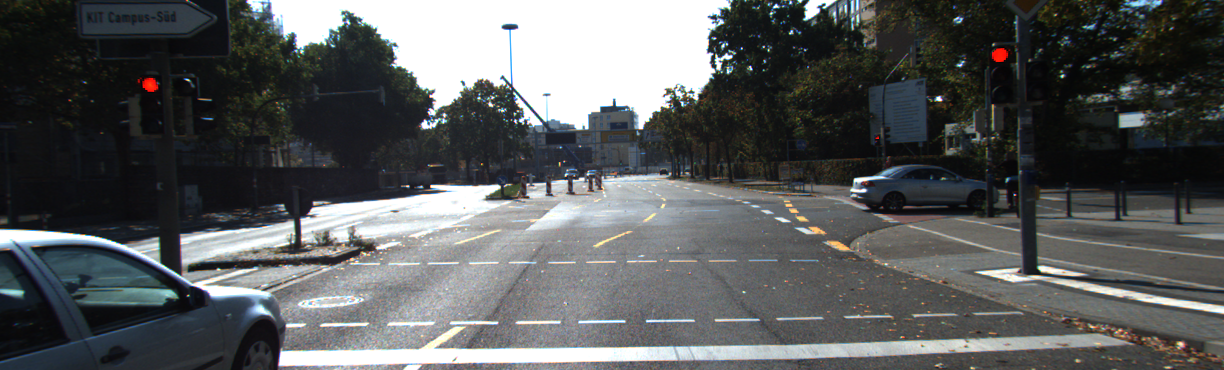
\includegraphics[width=.75\linewidth]{imgs/kitti.png}
	}
	\subcaptionbox{Sim10k\cite{johnsonroberson2017driving}}{
		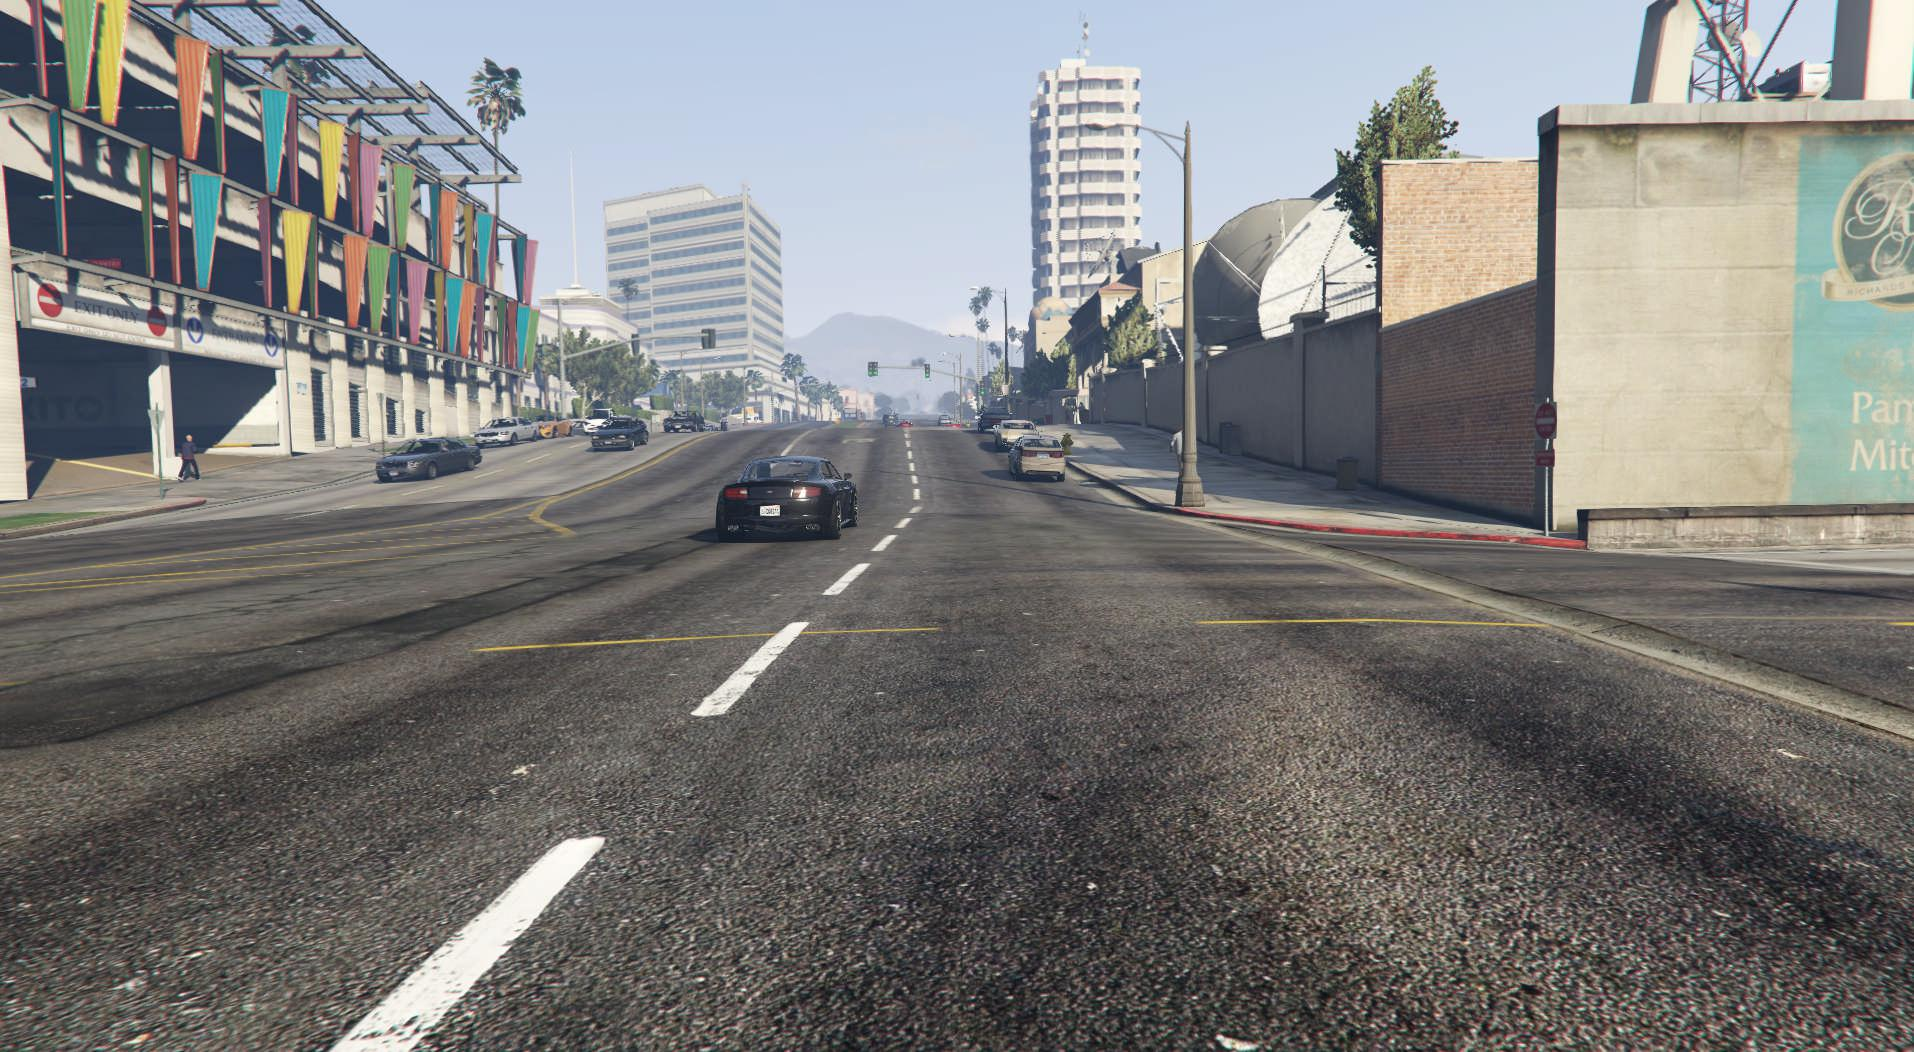
\includegraphics[width=.75\linewidth]{imgs/sim10k.jpg}
	}
	\caption{Examples of different street scenes datasets. It is evident that the appearance of images from different domains varies, even though they contain the same categories of objects. Indeed, images can be taken from different cameras and in different lightning or weather conditions. More extremely, \textit{Sim10k} only contains computer generated images: the texture of the objects widely differ from the ones in the other datasets.}
	\label{fig:datasets}
\end{figure}

\subsubsection{Anchor boxes}\label{sec:anchor}
In most cases, generating many possible bounding boxes is too cumbersome and leads to inaccurate predictions. If we already know which classes we want to detect, it may be more efficient to define a-priori a set of possible aspect ratios and zoom factors for the bounding boxes. For example, if we are interested in detecting cars, wide \textit{anchor boxes} can be defined at different scales, to identify both near and far objects of car shape.

As mentioned in Section~\ref{sec:fasterrcnn}, anchor boxes were first introduced for the \gls{rpn} of Faster \gls{rcnn} and were one of the main source of improvements in detection performances and speed\cite{ren2016faster}. The basic working schema is reported in Figure~\ref{fig:rpn}. Nowadays, anchor boxes are used in most architectures for object detection, such as \gls{yolo}, \gls{ssd} and RetinaNet. From an anchor boxes point of view, the difference between one-step and two-step methods is that the former analyze each anchor box independently, then refine and return only the most promising ones, while the latter start from the anchor boxes to estimate the true bounding boxes of the objects in the images.

\begin{figure}[tb]
	\centering
	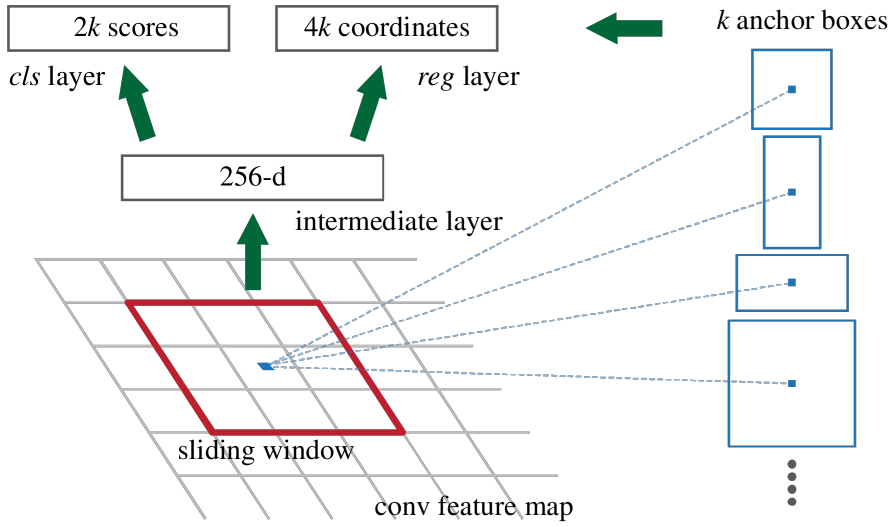
\includegraphics[width=.7\linewidth]{imgs/rpn.png}
	\caption{Anchor boxes, as used in Faster \gls{rcnn}'s \gls{rpn}\cite{ren2016faster}. At each position of the input image, $k$ bounding boxes with different scales and aspect ratios are proposed and forwarded to the rest of the network for evaluation.}
	\label{fig:rpn}
\end{figure}

\subsubsection{Non-maximum suppression}
Object detection models usually produce more than one detection for each object, which is not desirable. \Gls{nms} is a method to select one of many overlapping bounding boxes. For a set of overlapping boxes, the one predicted with the highest confidence is selected and all remaining boxes whose \gls{iou} with the chosen bounding box is over a certain threshold are discarded. In this way, only the most probable detection is kept for each object. An example is reported in Figure~\ref{fig:nms}.

\begin{figure}[tb]
	\centering
	\subcaptionbox{Before \acrlong{nms}}{
		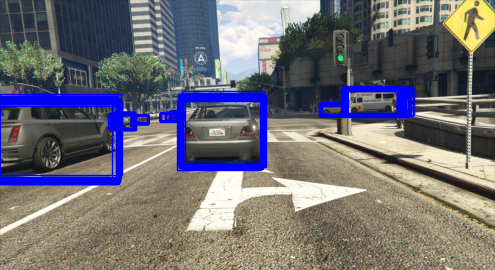
\includegraphics[width=.70\linewidth]{imgs/no_nms.png}
	}
	\subcaptionbox{After \acrlong{nms}}{
		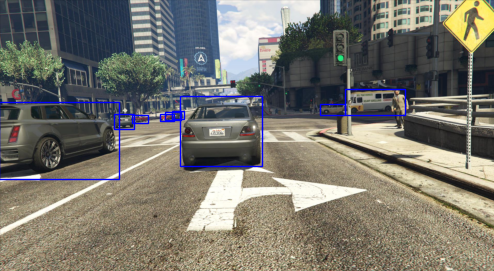
\includegraphics[width=.70\linewidth]{imgs/nms.png}
	}
	\caption{Example of application of \acrlong{nms} on a Faster \gls{rcnn} detector: several bounding boxes are proposed for each detected car, but only one per object is returned.}
	\label{fig:nms}
\end{figure}


\section{Domain adaptation}
For most use cases, a huge number of annotated images are necessary to train robust and efficient deep learning models. In an industrial context, the process of collecting and annotating data suitable for each specific customer case is often too expensive and time-consuming. In contrast, synthetic data can be generated through various rendering software, even free and open-source, easily and in massive quantities, for simulating the environments in which the models will be applied. However, deep learning models are effective if the training and test data are drawn from the same data distribution, so a model trained on simulated data is likely to perform badly on real data. Domain adaptation techniques can be used to transfer the knowledge acquired on the \textbf{source domain} (e.g., synthetic data) to the \textbf{target domain} (e.g., real data) without training a new model on the latter. In a domain adaptation setting, the task to be performed on source and target domains and the classes to be predicted remain the same, while the domain differs.

\bigskip
Domain adaptation methods are effective for several computer vision tasks, therefore dealing with image classification, object detection and semantic segmentation. In addition to the knowledge transfer from synthetic to real images, among other cases they can be used to adapt a model to different cameras, different weather conditions and moments of the day (e.g. from sunny to rainy weather or from day to night) or from infrared to normal images.

Different types of domain adaptation can be identified, based on whether annotations are available or not for the target domain:

\begin{itemize}
	\item \textbf{Supervised domain adaptation}: labeled data are available for both source and target domains.
	\item \textbf{Semi-supervised domain adaptation}: labeled data are available for the source domain, but only some data from the target domain are actually labeled.
	\item \textbf{Unsupervised domain adaptation}: labeled data are available for the source domain, but no labeled data are available for the target domain. All data from the target domain is therefore unlabeled.
\end{itemize}
Moreover, domain adaptation can be classified as \textbf{homogeneous}, if the domains share the same feature space, or \textbf{heterogeneous}, if features differ.

\medskip
Domain adaptation is mostly studied in the unsupervised and homogeneous scenario, with one source and one target domain.

\subsection{Domain adaptation methods}
Different approaches to the problem have been proposed in recent years. The most frequent ones are \textit{domain-invariant feature learning} and \textit{domain mapping}.

\subsubsection{Domain-invariant feature learning}
Several methods try to align source and target domains by creating a domain-invariant feature representation at the level of the neural network for feature extraction. Intuitively, if a model performs well on domain-invariant features extracted from the source domain, it should generalize to the target domain since the two distributions are aligned. A schema is reported in Figure~\ref{fig:align}.

\begin{figure}[ht]
	\centering
	\subcaptionbox{Training}{
		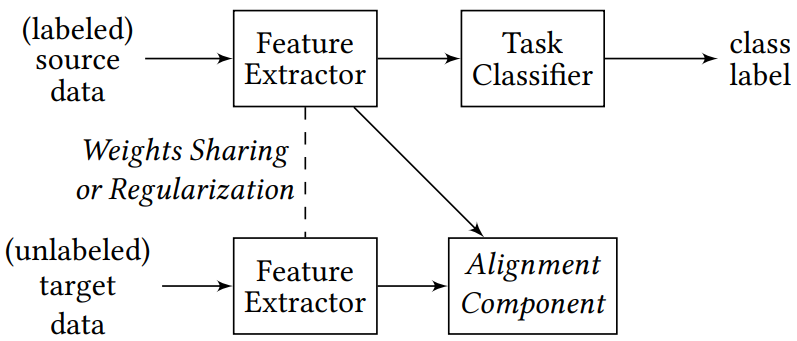
\includegraphics[width=.47\linewidth]{imgs/align_train.png}
	}
	\subcaptionbox{Testing}{
		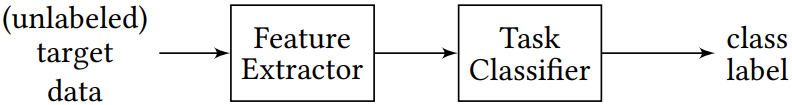
\includegraphics[width=.47\linewidth]{imgs/align_test.png}
	}
	\caption{General schema for domain-invariant feature learning\cite{wilson2020survey}}
	\label{fig:align}
\end{figure}

Methods following this approach differ in how they align the domains. An adversarial approach, as in \glspl{gan}, is often used through a domain classifier which outputs whether the features extracted by the \gls{cnn} belong to source or target domain. At the same time, the feature extractor is trained with the aim of fooling the domain classifier, so that it is unable to correctly classify from which domain the feature representation originates. The two networks are trained simultaneously and in an adversarial fashion.

\subsubsection{Domain mapping}
An alternative to creating domain-invariant feature representations is mapping one domain to the other, making source images similar to the target or vice versa. For example, synthetic images from \textit{Sim10k} can be mapped to the real world, transferring them to the \textit{CityScapes} style. This can be obtained with conditional \glspl{gan} for image-to-image translation that do not take into account the annotations of source images. Therefore, domain adaptation can be accomplished by training a \gls{gan} to map data from source to target and then training a machine learning model on the mapped labeled source images (that can now be considered as belonging to the target domain). At test time, the model is used to make predictions on unlabeled target data. A general schema is reported in figure~\ref{fig:gan}. However, \gls{gan} training is challenging and may incur in several problems such as mode collapse, when a generative network learns to only produce a limited amount of output images.

\begin{figure}[ht]
	\centering
	\subcaptionbox{Training}{
		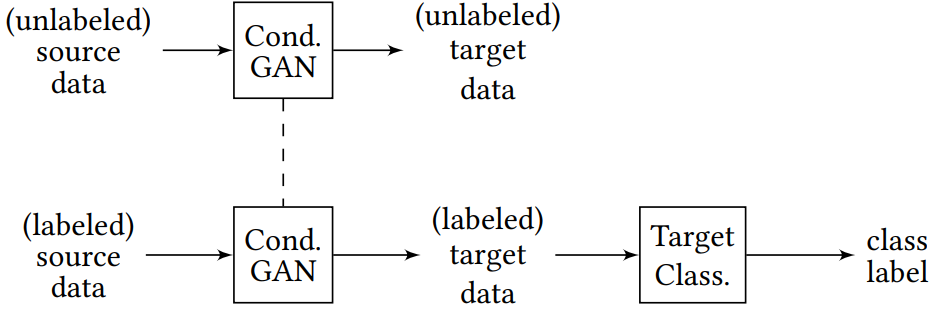
\includegraphics[width=.605\linewidth]{imgs/gan_train.png}
	}
	\subcaptionbox{Testing}{
		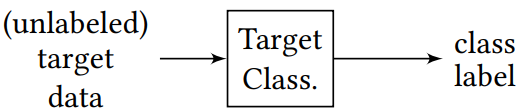
\includegraphics[width=.335\linewidth]{imgs/gan_test.png}
	}
	\caption{General schema for domain mapping\cite{wilson2020survey}}
	\label{fig:gan}
\end{figure}

\subsubsection{Previous works}
Several fundamental domain adaptation methods can be identified in the case of image classification. These methods have laid the foundation for many subsequent works.

\paragraph{Domain Adversarial Neural Network}\label{sec:dann}
\gls{dann}\cite{ganin2015unsupervised} is a classic method for unsupervised domain adaptation with the objective of learning domain invariant features. The network is composed of a standard feature extractor, a label predictor and a domain classifier: without this last component, it consists of a standard model for image classification.

The alignment between domains is achieved through the gradient reversal layer, introduced in this work: this layer leaves input unchanged during the forward step and reverses the gradient during backpropagation, multiplying it by a negative factor $-\lambda$. The network is trained adversarially, with the aim of minimizing the label predictor’s loss. 
At the same time, it also seeks the backbone parameters that maximize the domain classifier loss and the domain classifier parameters that minimize its own loss.

The objective is to align the two data distributions, fooling the domain classifier: when alignment is accomplished, the label predictor is capable of correctly classify an image, whether it is taken from the source or the target domain, while the domain classifier can only return random guesses. A network representation is reported in Figure~\ref{fig:dann}.

\begin{figure}[ht!]
	\centering
	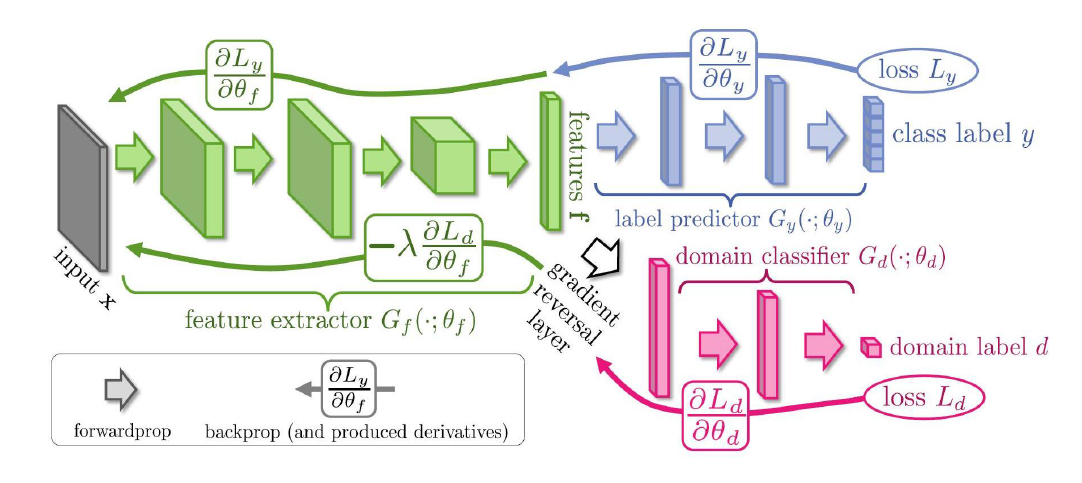
\includegraphics[width=0.95\linewidth]{imgs/dann.png}
	\caption{\gls{dann} architecture\cite{ganin2015unsupervised}}
	\label{fig:dann}
\end{figure}

\medskip
More formally and using the same notation as in Figure~\ref{fig:dann}, the aim is to find the values of the parameters $\theta_f$, $\theta_y$ and $\theta_d$ that minimize the following function:
\begin{equation}
	E(\theta_f, \theta_y, \theta_d) = \sum_{
		\substack{i=1\ldots N\\d_i=0}
	}L^{i}_{y}\left(\theta_f, \theta_y\right) - 
	\lambda \sum_{i=1\ldots N}L^{i}_{d}\left(\theta_f, \theta_d\right).
	\label{eq:dann}
\end{equation}
In~\eqref{eq:dann}, $L_y$ and $L_d$ are the objective functions for label and domain prediction respectively: $L^{i}_{y}$ and $L^{i}_{d}$ are computed for the $i$-th training image. By mapping the source and target domains to $0$ and $1$ respectively, the condition $d_i=0$ in the first sum implies that the label classifier is trained only if the network receives annotated images from the source domain.

$\lambda$ is therefore the only additional hyperparameter with respect to the training of a standard classification model and its value is to be fixed a priori. To increase the stability of the training and to foster good learning of the domain classifier at the beginning of the training procedure, $\lambda$ is sometimes set dynamically. The following expression can be used to change its value from $0$ (at the beginning of the procedure) to $1$ (at the end) according to the training progress represented by $p$ (in turn between $0$ and $1$):
\begin{equation}
	\lambda_p = \frac{2}{1 + \exp{\left(-\gamma\cdot p\right)}} - 1.
	\label{eq:dynamic_lambda}
\end{equation}
This avoids the need to seek the optimal value for $\lambda$, but introduces the new hyperparameter $\gamma$ (which represents the speed at which the value of $\lambda_p$ converges to 1).

\paragraph{Adversarial Discriminative Domain Adaptation}\label{sec:adda}
\gls{adda}\cite{tzeng2017adversarial} is an adversarial method like \gls{dann}, but is composed of three consecutive phases:
\begin{enumerate}
	\item \label{item:adda1} A \gls{cnn} is trained on labeled source examples in order to learn a feature representation for the source domain that can be successfully identified by a classifier. This source \gls{cnn} is frozen.
	
	\item \label{item:adda2} Adversarial adaptation is then performed.
	The objective is to train a feature extractor for the target domain: features extracted from the target domain have to be aligned to the ones extracted by the feature extractor trained at step~\ref{item:adda1} on images belonging to the source domain. A domain discriminator that receives features extracted by the aligned feature extractor from an image belonging to the target domain should therefore state that these features are extracted from an image of the source domain instead.
	%The objective is to train a target feature extractor in a way that a discriminator which receives features extracted from the two domains cannot predict their domain label, in order to align the domain representations.
	
	This is done through \quotes{flipped labels}: the training procedure fools the domain discriminator into believing that the features extracted from the target domain belong to the source domain instead. As a consequence, the target feature extractor is lead to learn features for the target domain that the domain discriminator could misclassify (as belonging to the source domain).
	
	\item For inference on images belonging to target domain, the aligned feature extractor (trained at step~\ref{item:adda2}) is used to extract features that now belong to the shared feature space. These features are then classified by the classifier that was previously trained on the source domain (in step~\ref{item:adda1}).
\end{enumerate}
A method overview is reported in Figure~\ref{fig:adda}.

\begin{figure}[ht!]
	\centering
	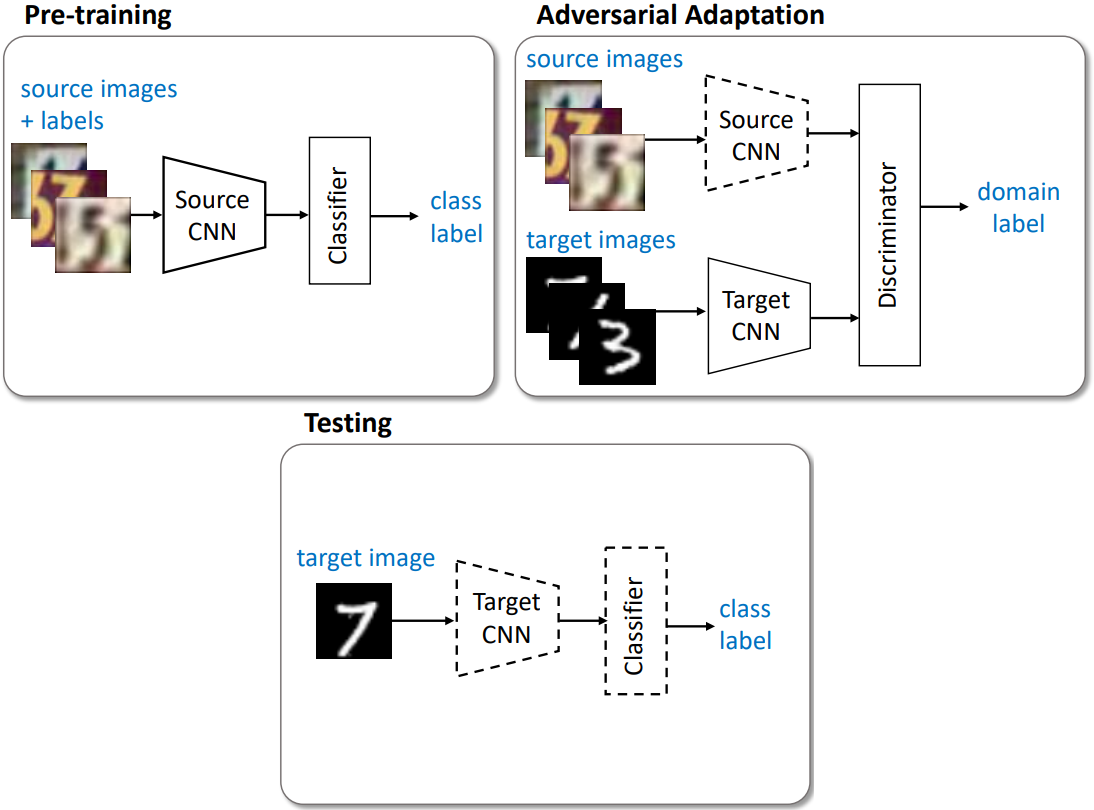
\includegraphics[width=.75\linewidth]{imgs/adda.png}
	\caption[\acrshort{adda} working schema]{\acrshort{adda} working schema\cite{tzeng2017adversarial}. The dashed lines indicate the parts of the networks that are previously learned and now frozen, while the network learns the remaining parameters.}
	\label{fig:adda}
\end{figure}

\paragraph{Enhancing photorealism enhancement}
It is worth mentioning a domain mapping approach, recently proposed by Richter \textit{et al.}\cite{richter2021enhancing}, for generating photorealistic images from computer games. Synthetic images, taken for example from the video-game \textit{Grand Theft Auto 5}, are processed in a way that they look realistic, following the camera and lightning conditions of real street scenes datasets such as \textit{CityScapes} or \textit{\gls{kitti}}. Resulting images are adapted to the data distribution of the dataset containing real-world images and can be used to train machine learning models for any computer vision task. The model can then be evaluated and applied on real data that the model has never seen. A few examples are reported in Figure~\ref{fig:photorealism}.

\begin{figure}[ht!]
	\captionsetup[subfigure]{labelformat=empty}
	\centering
	\begin{subfigure}{.47\textwidth}
		\centering
		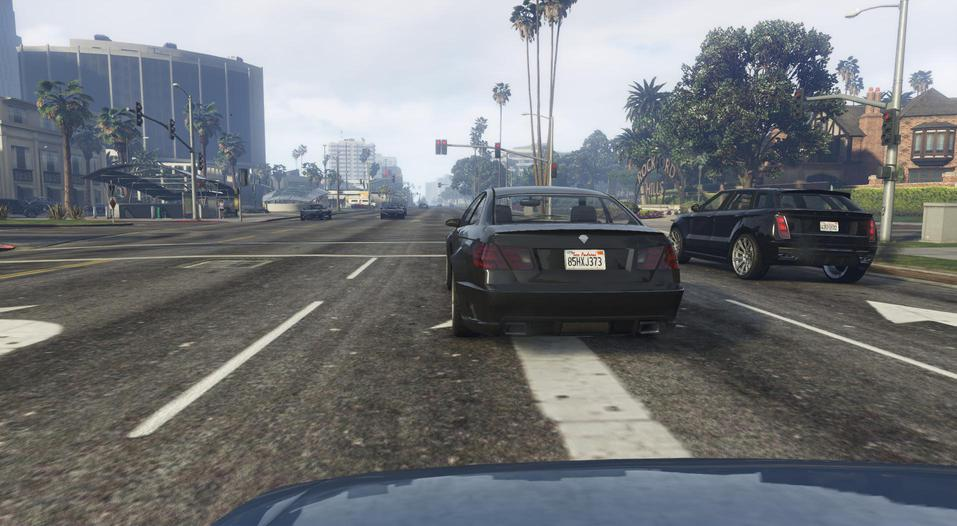
\includegraphics[width=\textwidth]{imgs/gta1.jpg}
	\end{subfigure}%
	\hspace{.02\linewidth}
	\begin{subfigure}{.47\textwidth}
		\centering
		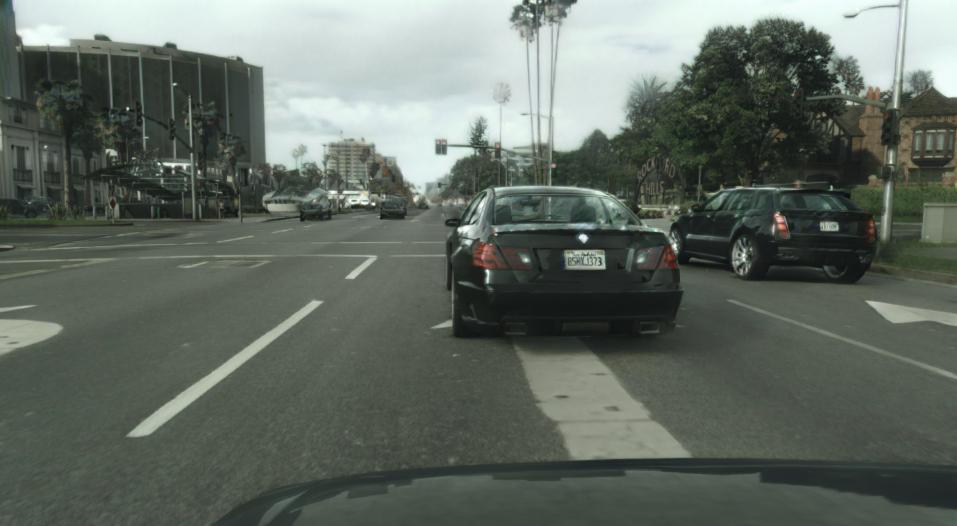
\includegraphics[width=\textwidth]{imgs/res1.jpg}
	\end{subfigure}\\
	\begin{subfigure}{.47\textwidth}
		\centering
		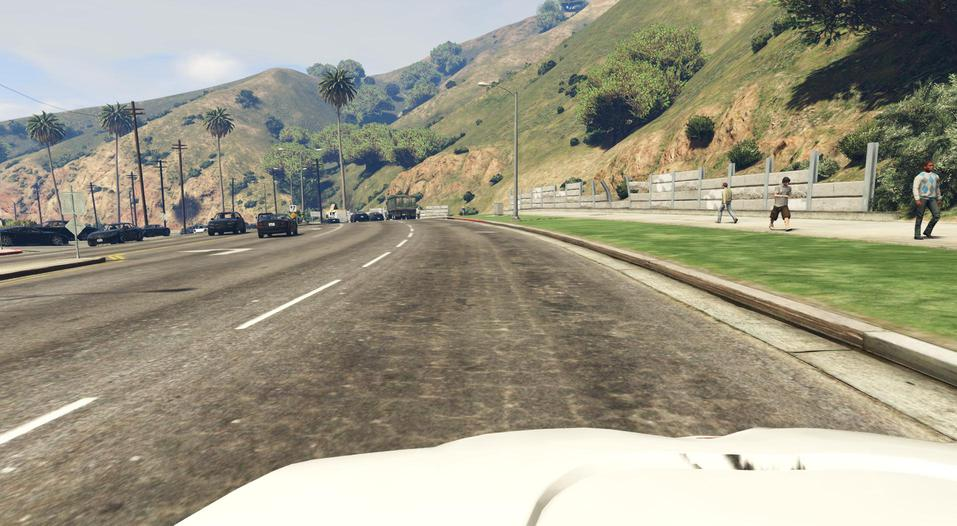
\includegraphics[width=\textwidth]{imgs/gta2.jpg}
	\end{subfigure}%
	\hspace{.02\linewidth}
	\begin{subfigure}{.47\textwidth}
		\centering
		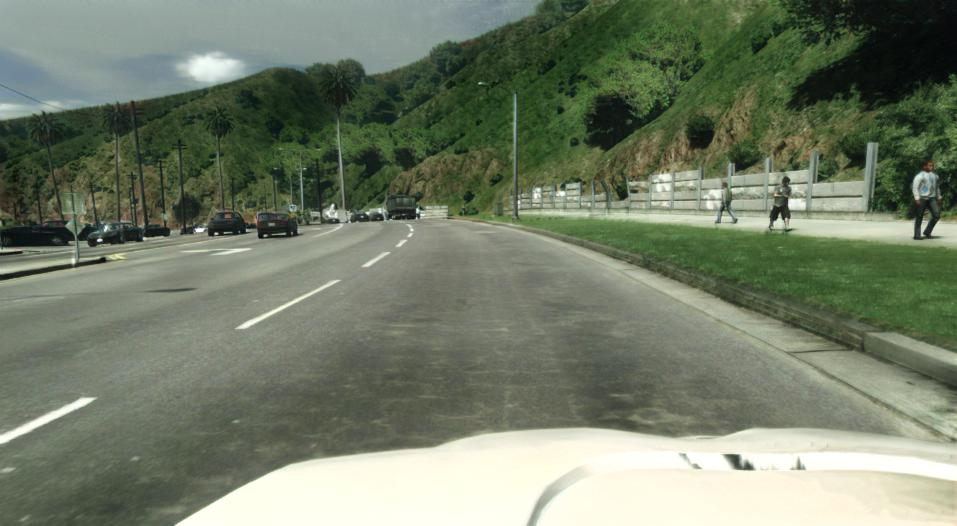
\includegraphics[width=\textwidth]{imgs/res2.jpg}
	\end{subfigure}
	\caption{Examples of application of photorealism enhancement of images from the video-game \textit{GTA 5} (left), to mimic the style of the \textit{CityScapes} dataset (right)\cite{richter2021enhancing}}
	\label{fig:photorealism}
\end{figure}

In this work, photorealism enhancement is performed starting from a set of intermediate buffers, called \textit{G-buffers}, that are produced by game engines during the rendering process. These buffers are extracted from the computer graphics pipeline and contain information about geometry, materials, and lightning in the scene. It is therefore required to have access to these low-level elements. After extraction, they are fed to an \textit{image enhancement} \gls{cnn}, with the goal of adapting image features.

\medskip
The image enhancement network is trained jointly with two objectives:
\begin{itemize}
	\item a \gls{lpips} loss, first introduced by Zhang \textit{et al.}\cite{zhang2018unreasonable}, is used to penalize large structural differences between the rendered and the enhanced images;
	\item a discriminator network is trained to discern between real and synthetic enhanced images and is used to evaluate the realism of adapted images.
\end{itemize}

In addition, a sampling strategy is followed to select synthetic and real image patches with similar content. The full training procedure allows reducing visual artifacts and providing temporally stable results.

%\paragraph{Asymmetric Tri-Training}
%Differently from the previous mentioned methods, asymmetric tri-training\cite{saito2017asymmetric} performs adaptation through pseudo-labelling. Three networks, sharing the same feature extractor, are used. Two of them include a classifier trained on source labeled images, with the aim of classifying features extracted from target image. If their predictions are coherent and with high confidence, the predicted pseudo-labels are assigned to those images. The third network is then trained with those pseudo-labels. An additional \gls{loss} is used to force a different point of view for the two source classifiers.

\subsection{Domain adaptation for object detection}
Like classification models, object detectors suffer from domain shifts between different datasets, which can lead to drastic performance degradation. Annotating images for an object detection task is even more expensive and time-consuming than classification, since each image may contain more than one object that needs to be assigned a bounding box and object category. Due to the different nature of the problem, direct translation of domain adaptation methods for classification may not be effective, and ad-hoc methods have been proposed, generally based on existing object detectors.

\subsubsection{Previous works}
\paragraph{Domain Adaptive Faster R-CNN}\label{sec:dafrcnn}
Domain Adaptive Faster \gls{rcnn}\cite{chen2018domain} is one of the first works to tackle the problem of cross-domain object detection. It uses a Faster \gls{rcnn} as base object detector and the network is trained with adversarial adaptation with gradient reversal layers at different levels. Indeed, in an object detection scenario the domain shift can occur at high level, such as image style and illumination, and at low level, such as object appearance and bounding box size. The former is referred to as \textit{image level}, while the latter is defined as \textit{instance level}. An additional loss function, referred as \textit{consistency loss}, is used to enforce consistent predictions from the two domain classifiers.

At inference time, the aligned Faster \gls{rcnn} is normally used.

\paragraph{Strong-Weak Distribution Alignment}
Aligning image level features as in Domain Adaptive Faster \gls{rcnn} makes the strong assumption that image components, such as backgrounds and scene layouts, must be similar across domains in addition to object categories. In the case of large domain shifts, that may affect the model performances. Saito \emph{et al.}\cite{saito2019strongweak} propose a weak global alignment (at image level) combined with a strong alignment of local features (such as texture or color of the objects in the two domains), which are most likely to be similar.

For weak alignment between domains, the domain classifier should focus on examples that are hard to classify, so near the boundaries between the two data distributions. This can be achieved using the focal loss to train the domain classifier, in order to tune the importance of source or target images whose domain is easy to predict.

\paragraph{Progressive Domain Adaptation}
Hsu \emph{et al.}\cite{hsu2019progressive} introduce an intermediate domain between source and target, exploiting a \gls{gan} to map source images in the target domain. Adaptation is performed in two steps, from source to intermediate and then from intermediate to target, in order to introduce a bridge between source and target domains. That helps to reduce the domain shift and simplifies the adaptation process, such that an object detection model can be trained on the intermediate domain. In addition, a weight is assigned to generated data, giving more importance to images that are closer to the target distribution.

When adaptation between the source and the intermediate domains is completed, the aligned model can be used for inference on unlabeled images from the target domain.

\paragraph{Domain Adaptive RetinaNet}\label{sec:daretinanet}
Recently, Pasqualino \emph{et al.}\cite{pasqualino2020unsupervised} proposed an adaptation approach for the RetinaNet model, but that can be applied to any architecture that includes a \gls{fpn} backbone. Different domain discriminators with different architectures are applied at different levels of the \gls{resnet} backbone which is used to construct the feature pyramid, with gradient reversal layers. In this way, extracted features are aligned at different levels in the backbone and the representation derived by the \gls{fpn} is coherent and meaningful.

\paragraph{Image statistics matching}\label{sec:kis}
The method introduced by Abramov \emph{et al.}\cite{abramov2020simple} relies on image transformations at pixel level instead of adversarial techniques or complex architectures. The objective is to transform annotated source images in a way to make them similar to the unlabeled target domain, matching color statistics and histograms. During training, a target image is randomly chosen for each image belonging to the source domain and the mean and covariance of its color channels are aligned, as well as its color histogram that are matched accordingly. In this way, a standard detection model can be trained on modified source image with annotations and directly applied on the target domain.

Similar approaches are commonly used in networks for style transfer, but in these cases the correspondence between source and target images is performed at the level of extracted features and not at image level.

%\blankpagestyle{headings}

%\lipsum[1-2]

\chapter{Method}
\section{Introduction}
This Master Thesis starts from the investigation of common approaches for domain adaptive object detection, in order to identify and possibly correct critical points and propose appropriate means of improvement.

\bigskip
A widespread belief is that extremely complex methods are more likely to achieve good performances than simple ones. Considering for example neural networks, the trend over the years has been to try making the networks deeper and deeper, which has produced extraordinary results but at the same time led to several problems in the training procedures. Recently, simple architectures like \textit{MLP-Mixer}\cite{tolstikhin2021mlpmixer} and \textit{Feed-Forward Stack}\cite{melaskyriazi2021need}, composed of \acrlongpl{mlp} only, reached surprisingly good performances in image classification.

A similar question can be raised for the problem of domain adaptation in an object detection scenario: can simple methods perform comparably or even better than the complex ones that are mostly studied in the literature? Indeed, in an industrial context engineers do not often have the time to deeply understand elaborate network architectures, potentially not useful for the problem they are facing, and must consider the trade-off between complexity and expected efficacy. Simple methods that are capable of reaching good performances are greedily researched and can boost their productivity.

\bigskip
These \quotes{simple} methods are mostly explored in this work. However, traditional domain adaptation methods, that deeply affect the network architecture, play an important role in research, and present unresolved issues that may undermine their use in actual engineering applications. Possible ways to address some detected issues are explored and tested, in parallel to the aforementioned simple approaches to domain adaptive object detection.

\bigskip
For the sake of completeness, the studied methods are implemented and tested on two popular object detection models presented in Section~\ref{sec:detection}, when they are compatible with both architectures: Faster \gls{rcnn} and RetinaNet.

\section{Data augmentation for domain randomization}\label{sec:dataaug}
Data augmentation is a widely used technique to ease the training of deep learning models and improve their generalization capability. In a typical application, different transformations are randomly applied on training images, in order to vary their appearance and virtually introduce new data on which a model can learn.

Data augmentations can modify the orientation of the images or operate at pixel level, transforming their color and appearance. Those operations can be geometric, if they geometrically distort the image without modifying its content, or color-based, if they distort color channels without modifying the position of the pixels. Common transformations include, but are not limited to, horizontal and vertical flip, rotation, translation and color shift. For an object detection task, bounding boxes have to be updated coherently with the applied geometric data augmentation.

\begin{figure}[ht!]
	\centering
	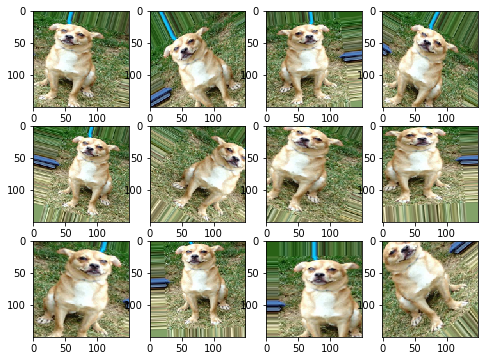
\includegraphics[width=0.8\linewidth]{imgs/augmentation.png}
	\caption{A few examples of data augmentation}
	\label{fig:augmentation}
\end{figure}

Therefore, data augmentation techniques can extensively alter the image appearance. If a model is trained with high-impact data augmentation on labeled images from a domain, it can potentially achieve good results on a different domain it has never seen. That falls in the case of \textbf{domain randomization}: training images are drawn from a data distribution which is way larger than the original one, so the model can learn to generalize to different domains. In some ways, the network is \quotes{overwhelmed} with different versions of the same images, in order to recognize their contents in different conditions. For domain adaptation, the resulting data distribution can possibly include the target domain or intermediates domains that are closer to the target domain than the source domain. Intuitively, performances on non-augmented images drawn from the source domain decrease as the data distribution gets larger, while the generalization capability to remote target domains increases.

\bigskip
Most works that investigate domain randomization focus on \textit{sim2real} knowledge transfer and address the problem generating a large variety of synthetic training images. The famous one by Tobin \textit{et al.}\cite{tobin2017domain} defines different randomization parameters that control, inter alia, position, number and type of the objects present in an image, as well as lighting and camera conditions. An interval of values is defined for each parameter and, for generating an image, each parameter is uniformly sampled within its range and used to control the generator. A detection model is then trained on the generated synthetic images and should be able to generalize to real images containing the same kind of objects. Examples are reported in Figure~\ref{fig:randomization}.

\begin{figure}[ht!]
	\centering
	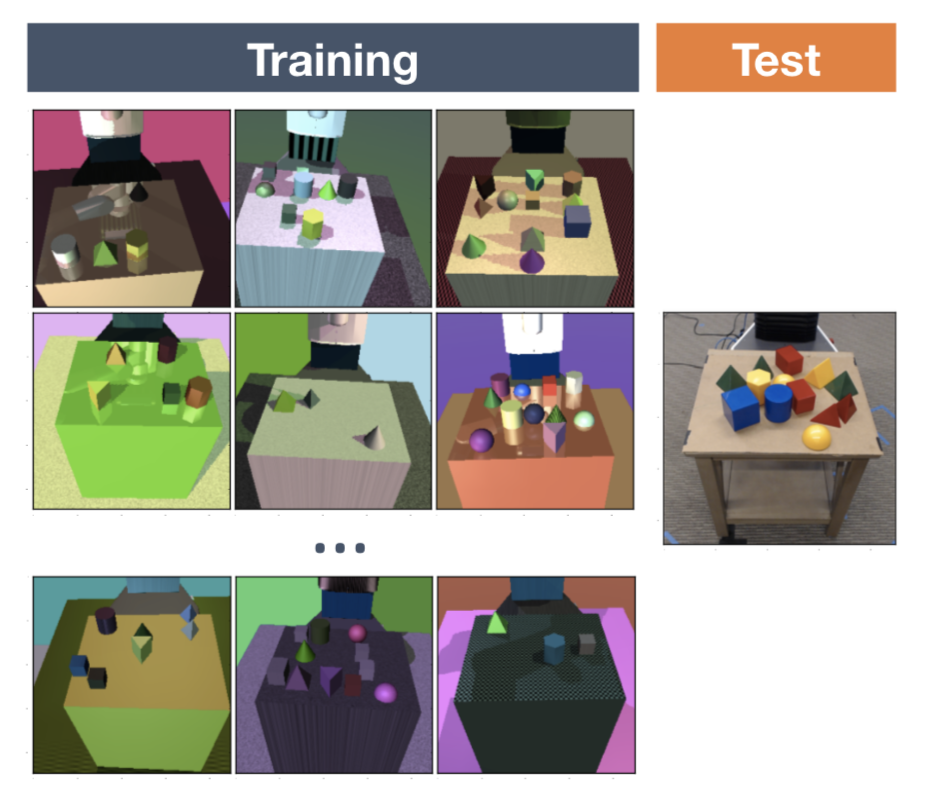
\includegraphics[width=0.7\linewidth]{imgs/randomization.png}
	\caption{Randomization in generating training images, in the framework proposed by Tobin \textit{et al.}\cite{tobin2017domain}}
	\label{fig:randomization}
\end{figure}

In the present work, instead, randomization is introduced through the combination of popular and commonly used operations for augmentation of image data, both geometric and color-based:
\begin{itemize}
	\item \textit{Horizontal flip}: geometric transformation that horizontally mirrors the image.
	\item \textit{Rotation}: geometric transformation that rotates image and bounding boxes of a degree value, sampled from a provided interval.
	\item \textit{Translation}: geometric transformation that horizontally and vertically translates image and bounding boxes of a given number of pixels, sampled from a provided interval.
	\item \textit{Shearing}: geometric transformation that deforms the image in a parallelogram shape according to horizontal or vertical axis. Horizontal and vertical shearing degrees are sampled from a provided interval.
	\item \textit{Color jitter}: color-level transformation that changes brightness, contrast, saturation and hue of the image. Jitter factors for each of the properties are sampled from provided intervals.
	\item \textit{Solarization}: color-level transformation that, for an image, inverts the color of all pixels whose value is above a threshold. The threshold is sampled from a provided interval.
	\item \textit{Equalization}: color-level transformation that equalizes the color histogram of the image.
\end{itemize}
The operations can be easily implemented and used in most popular deep learning frameworks.

\medskip
Many other operations are often used for data augmentation, but are not included in the performed experiments due to time constraints and since the possible combinations of the aforementioned operations are already numerous. An example is \textit{cutout}, which randomly masks regions of the training images in order to improve networks' robustness. Other operations, such as \textit{vertical flip}, do not make any sense in this context. Indeed, vertical flip would completely change the appearance of objects and background, leading to scenes that can never (or extremely rarely) appear in the real or simulated world.

\begin{figure}[ht]
	\centering
	\subcaptionbox{Original \textit{Sim10k} image}{
		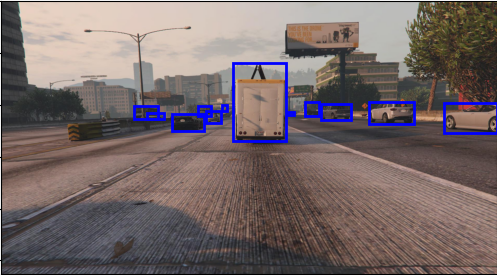
\includegraphics[width=.75\linewidth]{imgs/sim10korig.png}
	}\\
	\subcaptionbox{\textit{Sim10k} image with random augmentations}{
		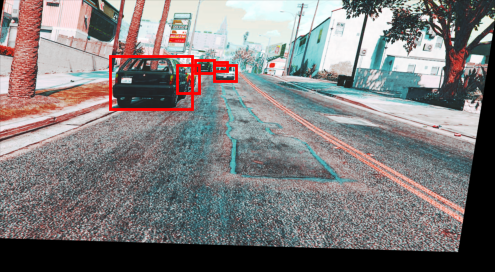
\includegraphics[width=.75\linewidth]{imgs/sim10kaug1.png}
	}
	\caption{Comparison between original and transformed images}
\end{figure}
\begin{figure}[ht]\ContinuedFloat
	\centering
	\subcaptionbox{\textit{Sim10k} image with random augmentations}{
		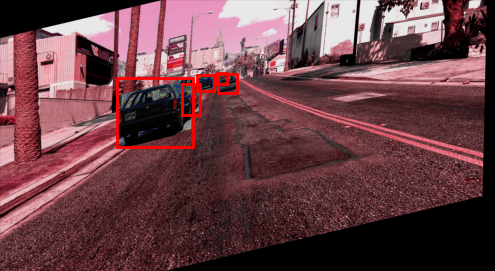
\includegraphics[width=.75\linewidth]{imgs/sim10kaug2.png}
	}\\
	\subcaptionbox{\textit{Sim10k} image with random augmentations}{
		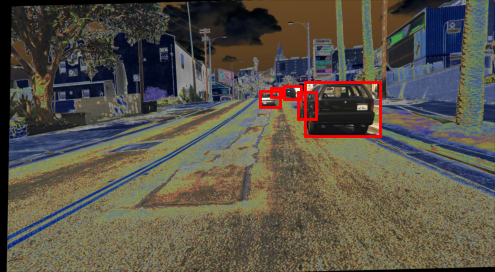
\includegraphics[width=.75\linewidth]{imgs/sim10kaug3.png}
	}
	\caption{Comparison between original and transformed images (cont.)}
	\label{fig:augs}
\end{figure}

\bigskip
More advanced data augmentation techniques, first introduced by Zoph \textit{et al.}\cite{zoph2019learning}, are specifically designed for the object detection task: they take into account the bounding boxes and only apply data augmentation operations to the objects they contain or to the background. The original work aims at finding the best combination of data augmentation operators, given the task and the training data. This combination is sought with reinforcement learning and should lead to the best performances when training a model for image classification or object detection. A few examples of the proposed transformations are reported in Figure~\ref{fig:learndataaug}.

\begin{figure}[ht!]
	\centering
	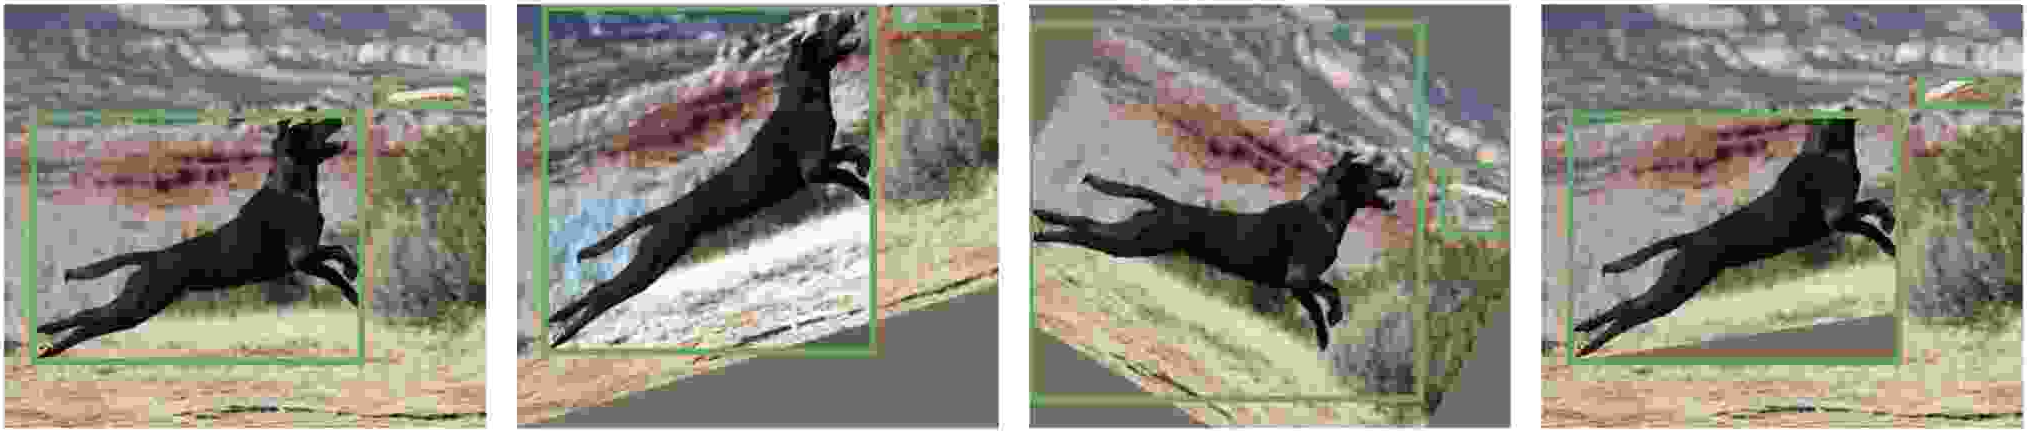
\includegraphics[width=0.9\linewidth]{imgs/learndataaug.png}
	\caption{Examples of usage of the data augmentation operators introduced by Zoph \textit{et al.}\cite{zoph2019learning}}
	\label{fig:learndataaug}
\end{figure}

\medskip
In a data randomization scenario, the data augmentation operators presented in the aforementioned work can be exploited to increase the variability of training images and widen the data distribution associated to the source domain. However, these peculiar transformations have to be used carefully: geometric operations can lead to unintended results, if applied to bounding box content or to background only. For example, if the bounding box is small and its content is translated horizontally, the object may disappear if the number of translated pixels is too high (see, for example, Figure~\ref{fig:objecttranslation}). Likewise, geometric transformations on background (the whole image except the content of bounding boxes) do not make sense, as they inevitably duplicate objects without associated bounding box. This bad behavior is clear in Figure~\ref{fig:backgroundrottransl}. In both cases, this would produce erroneous training images and lead to incorrect training procedures.

A few images produced by these wrong transformations are reported in Figure~\ref{fig:badaugs}.

\begin{figure}[ht]
	\centering
	\subcaptionbox{Original \textit{Sim10k} image}{
		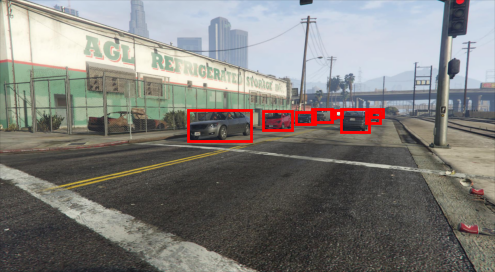
\includegraphics[width=.75\linewidth]{imgs/sim10korig2.png}
	}\\
	\subcaptionbox{Horizontal translation of objects inside bounding boxes\label{fig:objecttranslation}}{
		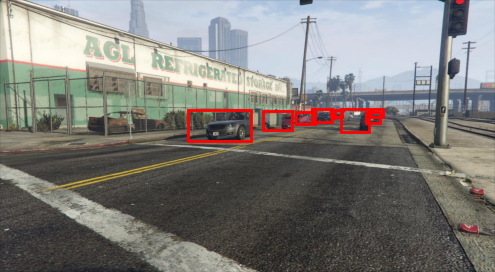
\includegraphics[width=.75\linewidth]{imgs/sim10kbadaug1.png}
	}
\caption{Examples of unsuccessful geometric transformations on bounding boxes or image background only}
\end{figure}
\begin{figure}[ht]\ContinuedFloat
	\centering
	\subcaptionbox{Rotation of objects inside bounding boxes}{
		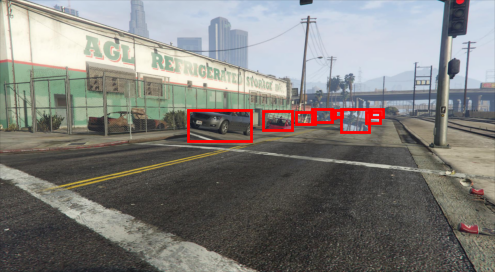
\includegraphics[width=.75\linewidth]{imgs/sim10kbadaug2.png}
	}\\
	\subcaptionbox{Rotation and translation of image background, keeping the objects in the original bounding boxes fixed\label{fig:backgroundrottransl}}{
		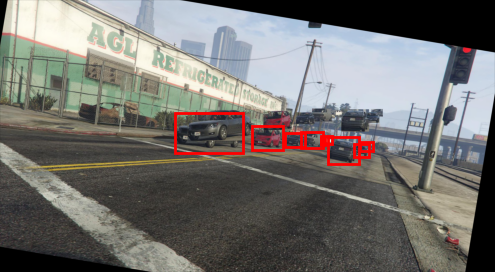
\includegraphics[width=.75\linewidth]{imgs/sim10kbadaug3.png}
	}
	\caption{Examples of unsuccessful geometric transformations on bounding boxes or image background only (cont.)}
	\label{fig:badaugs}
\end{figure}

\section{Adapting a two stage object detector}
Domain Adaptive Faster \acrshort{rcnn}\cite{chen2018domain}, presented in Section~\ref{sec:dafrcnn}, is without any doubt the most popular method designed to attain successful object detection in different domains. Since its introduction, the paper has been cited hundreds of times and several methods based on it have been proposed. It is therefore a good adaptation method to be used as baseline and for comparison with other architectures and methods.

The training process considers annotated images from the source domain and unlabeled images from the target domain at the same time. Adaptation is performed at two different levels  using the gradient reversal layers presented in Section~\ref{sec:dann}:

\begin{itemize}
	\item Image level: the features extracted by the network backbone are forwarded to a patch-based domain classifier. Such patch classifiers, introduce by Isola \textit{et al.}\cite{isola2018imagetoimage}, divide each feature map of an image into $ N\times N $ patches and classify them independently. For a domain classifier, each patch is classified as extracted from source or target domain. In this way, the importance of the global differences inside images is reduced and the classifier is trained more precisely. Adaptation at this level aims at reducing the global differences such as image style and illumination.
	\item Instance level: the features extracted by the \gls{rpn} are passed to a domain discriminator before being fed to the label classifier and bounding box regressor for the final prediction. That helps to reduce differences related to the objects that appear in the images, such as object size, texture and viewpoint.
\end{itemize}
In addition, a consistency regularization is added to encourage similar predictions from the two domain classifiers. A method overview is reported in Figure~\ref{fig:dafasterrcnn}.

\begin{figure}[ht]
	\centering
	\includegraphics[width=\linewidth]{imgs/dafasterrcnn.png}
	\caption{Overview of the Domain Adaptive Faster \gls{rcnn} model\cite{chen2018domain}}
	\label{fig:dafasterrcnn}
\end{figure}

\bigskip
A training batch is composed of both source and target images and the training procedure is organized as follows:
\begin{itemize}
	\item When the network receives, as input, labeled images from the source domain, they are used to train both the base Faster \gls{rcnn} and the domain adaptation components.
	\item When the network receives, as input, unlabeled images from the target domain, they are only used to train the domain adaptation components. Indeed, unlabeled images are not useful for the base detector as object bounding boxes and class information are not available.
\end{itemize}
For inference, additional domain adaptation components are not considered and the standard Faster \gls{rcnn} with learned weights is used.

\section{Adapting the FPN}
\acrfull{fpn}, first introduced by Lin \textit{et al.}\cite{lin2017feature}, is a cheap but effective method to increase the performances of a detection model. Nowadays, it is often included in the backbone network of object detectors such as Faster \gls{rcnn} and is one of the fundamental bricks of the RetinaNet model. One of the most popular computer vision frameworks for research, \textit{torchvision} by \textit{PyTorch}\cite{paszke2019pytorch}, only provides pretrained backbones with \gls{fpn} for Faster \gls{rcnn} models. Therefore, using \gls{fpn} for object detection problems is straightforward and highly performing with respect to standard backbones without \glspl{fpn}, that are rarely or never used in real applications.

However, the \gls{fpn} architecture introduces some problems for adversarial feature alignment on the output of the backbone (such as the \textit{image} level in the Domain Adaptive Faster \gls{rcnn} model): backbone layers must be aligned in a way that the extracted feature pyramid representation is logical and coherent. Consider, for example, a case in which domain alignment is performed only on the last layer of the backbone: at the end of the training procedure, the features extracted from the last layer would be aligned between the domains, while the features extracted from the previous layers may not be so. As \glspl{fpn} construct rich feature representations by linking the features extracted from different backbone layers, that would lead to a meaningless feature pyramid.

\begin{figure}[ht]
	\centering
	\includegraphics[width=.6\linewidth]{imgs/fpn.png}
	\caption{\Gls{fpn} architecture\cite{chen2018domain}}
	\label{fig:fpn}
\end{figure}

\subsection{Implementation on RetinaNet}
Domain Adaptive RetinaNet, introduced in Section~\ref{sec:daretinanet}, takes into account adversarial domain adaptation for a one-stage object detector with \gls{fpn} backbone. More precisely, in the RetinaNet model the \gls{fpn} uses the features extracted from the last three layers of a \gls{resnet} to construct a rich and multiscale feature pyramid of three levels from an input image at single resolution. This representation is then forwarded to two separate fully convolutional subnetworks, in order to predict the probability of presence of an object in each anchor box and the bounding box locations.

\bigskip
As \glspl{fpn} return feature maps of different sizes, considering all of them at the same time for adaptation is not straightforward and may lead to non-optimal performances. Pasqualino \textit{et al.}\cite{pasqualino2020unsupervised} perform adaptation through three different domain classifiers with different architectures. They receive as input the features extracted from the three \gls{resnet} layers that are used to build the \gls{fpn} representation.

For adversarial alignment, the features are forwarded through gradient reversal layers as in \gls{dann} (described in Section~\ref{sec:dann}): the overall network is trained normally but the gradient resulting from the domain classifiers is multiplied by a negative factor $-\lambda$, as in \eqref{eq:dann}, during the backpropagation phase, in order to push the \gls{resnet} to extract domain invariant features that can be used to accurately detect objects in target images. This allows the model to preserve a meaningful feature pyramid while aligning the two data distributions.

\medskip
Labeled source images are used to train the whole network, while unlabeled target images only train the three domain classifiers. At test phase, the domain classifiers are plugged off and the adapted RetinaNet is normally used.

\subsection{Implementation on Faster R-CNN}\label{sec:adapt_fpn_fasterrcnn}
The addition of a \gls{fpn} component to the backbone of a Faster \gls{rcnn} model considerably improves detection performances. For example, the authors of the paper that introduced the \gls{fpn} method reported 3.7 \gls{ap} points improvement on the \gls{coco} dataset\cite{lin2017feature}. Thanks to the \gls{fpn}, \gls{rpn} receives a rich feature representation at different resolutions and is able to better identify candidate \glspl{roi} of higher quality. As it can achieve better results than the standard architecture without \gls{fpn} at a negligible price, Faster \gls{rcnn} with \gls{fpn} backbone is commonly used. 

\bigskip
If the base detector includes a \gls{fpn} component, adaptation at image level as in the Domain Adaptive Faster \gls{rcnn} method has to be reconsidered. Two possible solutions can be identified in order to align the feature representations between different domains:
\begin{itemize}
	\item Adaptation can be directly performed on features extracted by the \gls{fpn}. Different levels of the feature pyramid can be forwarded, one at a time, to a domain classifier through gradient reversal layer (Figure~\ref{fig:adapt_fpn}). The resulting domain losses can be summed or averaged across all levels. This way, the objective is to push the \gls{resnet} backbone to extract feature representations that can be used to build a feature pyramid which is independent of the domain of each input image.
	\item Similarly to what is done by Pasqualino \textit{et al.}\cite{pasqualino2020unsupervised}, it is otherwise possible to directly align the \gls{resnet} features that serve as input for the \gls{fpn}: if they are not dependent from the domain, neither the resulting pyramid representation will be. The last three \gls{resnet} layers are therefore used to build the feature pyramid and are forwarded to three different domain classifiers with different architectures, through gradient reversal layers for adversarial alignment (Figure~\ref{fig:adapt_resnet}).
\end{itemize}
Such approaches have not yet been followed in the academic literature for two stage object detectors. In both cases, object detection network and domain adaptation components are trained jointly.

\begin{figure}[ht]
	\centering
	\subcaptionbox{Adversarial alignment on pyramidal feature representations, built by the \gls{fpn} from \gls{resnet} layers\label{fig:adapt_fpn}}{
		\includegraphics[width=.6\linewidth]{imgs/adapt_fpn.png}
	}\\
	\subcaptionbox{Adversarial alignment on features extracted by ResNet layers\cite{pasqualino2020unsupervised}\label{fig:adapt_resnet}}{
		\includegraphics[width=.6\linewidth]{imgs/adapt_resnet.png}
	}
	\caption{Approaches to adversarial domain adaptation at image level for an architecture with \gls{fpn}}
\end{figure}

The presence or absence of the \gls{fpn} in the backbone has no impact on adaptation at instance level, as \gls{rpn} returns \glspl{roi} in the same format. If different domain classifiers are used, the consistency regularization loss is independently computed for each \gls{resnet} layer between the domain prediction and the prediction at instance level, unique at each iteration. Otherwise, training proceeds as previously described.

\section{Image statistics matching}
As discussed in Section~\ref{sec:dataaug}, data augmentation techniques that significantly modify the appearance of images taken from a specific domain extend their data distribution, possibly covering several domains. A model can be trained on transformed images from the source domain without any architectural modification, possibly performing well on images drawn from a target data distribution.

\bigskip
Likewise, domain mapping methods transform images from a source domain in a way that a model can confuse them with images from the target domain: they focus on accurate modifications of images rather than upgrading base architectures. That is typically attained through \glspl{gan} for style transfer, but training of adversarial networks is generally complicated and time-consuming. Instead, the method introduced by Abramov \textit{et al.}\cite{abramov2020simple} tries to \quotes{keep it simple}, by performing easy but effective operations at image level with the objective of matching image statistics between source and target domains.

More precisely, for each labeled image from the source domain, an unlabeled image belonging to the target domain is randomly selected. Two transformations are applied one after the other:
\begin{enumerate}
	\item Feature Distribution Matching: the first operation transforms the source image in a way that it obtains the same color mean and covariance of the target image, while keeping the image content. It works pixel-wise through \gls{pca} whitening with Singular Value Decomposition, in order to efficiently uncorrelate the distribution of image pixels.
	\item Histogram Matching: the second transformation is a common one in image processing. It manipulates the pixels of the source image in order to align the distributions of its color histograms to the ones of the target image.
\end{enumerate}
A sample application of the method is reported in Figure~\ref{fig:kis}.

A detection model is therefore trained on labeled mapped images that share statistics with target images and can thus be considered as belonging to the target domain. The model can then be directly used for inference on the target domain, without any additional operation.

\begin{figure}[ht]
	\centering
	\subcaptionbox{Source image}{
		\includegraphics[width=.47\linewidth]{imgs/src.png}
	}
	\subcaptionbox{Target image}{
		\includegraphics[width=.47\linewidth]{imgs/tgt.png}
	}\\
	\subcaptionbox{Feature Distribution Matching}{
		\includegraphics[width=.47\linewidth]{imgs/fdm.png}
	}
	\subcaptionbox{Histogram Matching}{
		\includegraphics[width=.47\linewidth]{imgs/hm.png}
	}\\
	\subcaptionbox{Combination of Feature Distribution Matching and Histogram Matching}{
		\includegraphics[width=.47\linewidth]{imgs/fdm_hm.png}
	}
	\caption{Results obtained through Feature Distribution Matching and Histogram Matching on a sample image. \textit{Sim10k} and \textit{CityScapes} are considered as source and target domains respectively.}
	\label{fig:kis}
\end{figure}

\medskip
Additionally, transformations can be applied on a patch basis, in order to locally match images from source and target domains. Aforementioned transformations can be performed on smaller regions of the images, in correspondence between source and target domain. This way, matching focuses on local features and is less dependent on the global appearance of selected images from the two domains. An example of application of patch-based Feature Distribution Matching and Histogram Matching is reported in Figure~\ref{fig:patchkis}.

\begin{figure}[ht]
	\centering
	\subcaptionbox{Source image}{
		\includegraphics[width=.47\linewidth]{imgs/src_2x2.png}
	}
	\subcaptionbox{Target image}{
		\includegraphics[width=.47\linewidth]{imgs/tgt_2x2.png}
	}\\
	\subcaptionbox{Feature Distribution Matching}{
		\includegraphics[width=.47\linewidth]{imgs/fdm_2x2.png}
	}
	\subcaptionbox{Histogram Matching}{
		\includegraphics[width=.47\linewidth]{imgs/hm_2x2.png}
	}
	\caption{Results obtained through $2\times 2$ patch-based Feature Distribution Matching and Histogram Matching on a sample image. \textit{Sim10k} and \textit{CityScapes} are considered as source and target domains respectively.}
	\label{fig:patchkis}
\end{figure}

\chapter{Experimental results}
\section{Experimental settings}
This chapter reports, compares and discusses the results obtained with the methods presented in the previous chapter. For coherence with previous works, \textit{Sim10k} and \textit{CityScapes} are respectively considered as source domain and target domains. Experiments deal therefore with \textit{sim2real} domain adaptation, training a model to recognize cars in a simulated world for detection in the real. Results are presented in terms of \gls{map} computed at \gls{iou} threshold of $ 0.5 $, separately for the experiments performed with RetinaNet and Faster \gls{rcnn} base detectors. Impact of data augmentation operations, in addition to domain adaptation methods, is also studied. All experiments have been conducted with the PyTorch deep learning framework and run on an NVIDIA GeForce RTX 2070 \gls{gpu} with 8 GB of memory.

\bigskip
In the following sections, the models indicated as \quotes{oracle} are trained and tested directly on the target domain (\textit{CityScapes} in the \textit{sim2real} context) using the base detectors and without applying any data augmentation technique, except for the simple horizontal flip. This represents an upper bound for domain adaptation performance. Such a model cannot be trained in real applications, as, in the common case of unsupervised domain adaptation, annotations are not available for the target domain.

\subsection{Data processing}
As said, \textit{Sim10k} and \textit{CityScapes} are considered as source and target domain, for unsupervised domain adaptation between synthetic and real image data. As mentioned in Section~\ref{sec:datasets}, the two dataset use different formats for storing bounding box annotations. The Python library \textit{Datumaru}\cite{datumaro} is therefore used to convert them into a common format.

\medskip
As an official Python interface is provided to easily load the annotations and compute the detection \gls{map}, the Microsoft \gls{coco} format has been chosen. Only annotations for the class \quotes{car} are kept, as this is the only common category in the two datasets containing street scenes.

\medskip
Finally, the open source tool \textit{cocosplit}\cite{cocosplit} is used to partition the \textit{Sim10k} dataset into training, validation and test sets with a proportion of 7\string:2\string:1, as standardized set splits are not officially available. The dataset is quite large (10000 annotated images) and it can be assumed that image distributions are similar between the three splits. On the other hand, splits are made public for \textit{CityScapes}, but annotations are not available for the test images. The performances of the tested domain adaptation methods are therefore evaluated on the provided validation set, as it is never used during training.

\medskip
When fed to the object detection models for training or evaluation, input images are resized so that the shortest side is equal to 600 pixels.

\subsection{Data augmentation}
Impact of data augmentation is extensively tested, for both domain randomization by itself or in combination with other methods for domain adaptation. The following parameters are used for each previously introduced data augmentation technique:
\begin{itemize}
	\item random rotation (\texttt{Rot.}) between $ -10 $ and $ 10 $ degrees;
	\item random translation (\texttt{Tr.}) between $ -100 $ and $ 100 $ pixels, independently chosen for the two axis;
	\item random shearing (\texttt{Sh.}) between $-20$ and $20$ degrees (not always used);
	\item brightness, contrast, saturation and hue randomly jittered (\texttt{C.J.}) between $ 0.5 $ and $ 1.5 $, independently chosen for each property;
	\item for solarization (\texttt{Sol.}), the threshold over which pixels are inverted is randomly sampled between $ 64 $ and $ 192 $ (with RGB pixel values going from $ 0 $ to $ 255 $ for each color channel).
\end{itemize}

Additional performed data augmentation techniques are horizontal flip (\texttt{HF}, a basic transformation which is always used) and equalization (\texttt{Eq.}). Both operations are parameter-free and are applied with probability 0.5 each.

Notations in parentheses are referred to when reporting the results in the next sections.

\bigskip
The Python library \textit{imgaug}\cite{imgaug} is exploited for data augmentation.

\subsection{RetinaNet}
The open-source RetinaNet implementation included in the PyTorch's library for computer vision (\textit{torchvision})\cite{torchvision_retinanet} has been used as starting point for the experiments with the base object detection model, which included domain randomization and image statistics matching. For Domain Adaptive RetinaNet, the implementation provided by the same authors of the original paper\cite{pasqualino2020unsupervised} using the \textit{detectron2} framework\cite{wu2019detectron2}\cite{daretinanet_github} is followed and adapted.

\bigskip
All used RetinaNet networks include a \gls{resnet}-50 backbone and are pre-trained on the \gls{coco} dataset. They are then finetuned on the data from one or both domains using the Adam optimizer for 15 epochs, with initial learning rate $1\times 10^{-4}$, reduced to $1\times 10^{-5}$ after 10 epochs. A training batch is composed of four annotated images from the source domain. When the target domain is needed for adversarial adaptation, two images are added to each training batch without considering image annotations, for a final batch size of 6.

\medskip
Additional configurations for RetinaNet include:
\begin{itemize}
	\item anchor boxes of size 32, 64, 128, 256 and 512 are generated with aspect ratios $0.5$, 1 and 2, for a total of 15 anchor boxes for each location of the feature map returned by the \gls{resnet} backbone;
	\item best 1000 bounding box proposals are kept before \gls{nms}, and only if detection confidence is greater than $0.05$;
	\item best 300 bounding boxes are returned after \gls{nms}, performed with \gls{iou} threshold $0.5$.
\end{itemize}

The focal loss hyperparameters, as in \eqref{eq:focalloss}, are set to $\alpha = 0.25$ and $\gamma = 2$.

When adversarial adaptation is applied on the last three layers of the \gls{resnet}-50 backbone (layers 3, 4 and 5), the $\lambda$ coefficient introduced in \eqref{eq:dann} evolves from 0 to 1, and is limited to $0.5$ for layers 3 and 4, and to $0.1$ for layer 5. The dynamic update is performed independently for each adversarial coefficient following the policy illustrated in \eqref{eq:dynamic_lambda}. In this last equation, $\gamma$ is set to 10.

\subsection{Faster R-CNN}
As for RetinaNet, \textit{torchvision}'s implementation of Faster \gls{rcnn} model is used as basic detector\cite{torchvision_fasterrcnn}. For Domain Adaptive Faster \gls{rcnn}, an implementation by the authors of the paper\cite{chen2018domain} is considered\cite{dafasterrcnn_github}, but is reimplemented in a more recent version of PyTorch and \textit{torchvision}. The original implementation is only used for testing the method without \gls{fpn}.

\bigskip
As for RetinaNet, all Faster \gls{rcnn} models include a \gls{resnet}-50 backbone and are pre-trained on \gls{coco}. Networks are then finetuned on \textit{Sim10k} (annotated) and \textit{CityScapes} (without annotations) for 15 epochs using the SGD optimizer with momentum of $0.9$ and weight decay of $5\times 10^{-4}$. Initial learning rate is set at $1\times 10^{-3}$ and is reduced to $1\times 10^{-4}$ after 10 epochs. In order to improve stability of two-stage object detectors, the learning rate is initialized using a warm-up policy. It is linearly increased from 0 to $1 \times 10^{-3}$ during the first 1000 training iterations.

Batch size of 4 is used when the model is trained only on annotated images from the source domain. When images from the target domain are used for adversarial domain adaptation the size of a training batch is 2: it is composed of one annotated image from the source domain and one unlabeled image from the target domain.

\medskip
Additional configurations for Faster \gls{rcnn} include:
\begin{itemize}
	\item anchor boxes of size 32, 64, 128, 256 and 512 are generated with aspect ratios $0.5$, 1 and 2, for a total of 15 anchor boxes for each location of the feature map returned by the \gls{resnet} backbone;
	\item during training, the \gls{rpn} extracts 1000 bounding box proposals after \gls{nms}, performed with \gls{iou} threshold $0.7$;
	\item during inference, 100 bounding boxes are returned after \gls{nms}, performed with \gls{iou} threshold $0.5$, and only if their detection confidence is higher than 0.05.
\end{itemize}

When adversarial domain adaptation is performed, the adversarial coefficient $\lambda$ is set to $0.1$.

\section{Domain randomization}
Table~\ref{table:rand_retinanet} and Table~\ref{table:rand_fasterrcnn} contain the results obtained by RetinaNet and Faster \gls{rcnn} (with \gls{fpn} backbone) respectively, trained on \textit{Sim10k} images using several data augmentation techniques and evaluated on \textit{CityScapes} test images. Images belonging to the target domain as considered as they are for evaluation, without applying any transformation. For each combination of data augmentation operations, the tables contain the detection \gls{map} on \textit{CityScapes}.

\begin{table}[tb]
	\centering
	\caption{\gls{map} with different data augmentation techniques for a RetinaNet model, trained on \textit{Sim10k} and evaluated on \textit{CityScapes}. Table columns indicate the transformations that are employed in each experiment. Only horizontal flip is used for the \quotes{oracle}.}
	\begin{NiceTabular}{cccccccc}
		\toprule
		HF & Rot. & Tr. & Sh. & C.J. & Sol. & Eq. & mAP@0.5 \\
		\midrule
		$\checkmark$ & & & & & & & 30.4   \\
		$\checkmark$ & $\checkmark$ & $\checkmark$ & & & & & 37.6   \\
		$\checkmark$ & $\checkmark$ & $\checkmark$ & $\checkmark$ & & & & 39.2   \\
		$\checkmark$ & $\checkmark$ & $\checkmark$ & & $\checkmark$ & & & 49.4   \\
		$\checkmark$ & $\checkmark$ & $\checkmark$ & & $\checkmark$ & $\checkmark$ & $\checkmark$ & \textbf{52.7}   \\
		$\checkmark$ & $\checkmark$ & $\checkmark$ & $\checkmark$ & $\checkmark$ & $\checkmark$ & $\checkmark$ & 49.8   \\
		\midrule
		\Block[l]{1-7}{Oracle} & & & & & & & 68.7   \\
		\bottomrule
	\end{NiceTabular}
	\label{table:rand_retinanet}
\end{table}

\begin{table}[tb]
	\centering
	\caption{\gls{map} with different data augmentation techniques for a Faster \gls{rcnn} model with \gls{fpn}, trained on \textit{Sim10k} and evaluated on \textit{CityScapes}. Table columns indicate the transformations that are employed in each experiment. Only horizontal flip is used for the \quotes{oracle}.}
	\begin{NiceTabular}{ccccccc}
		\toprule
		HF & Rot. & Tr. & C.J. & Sol. & Eq. & mAP@0.5 \\
		\midrule
		$\checkmark$ & & & & & & 46.3   \\
		$\checkmark$ & $\checkmark$ & $\checkmark$ & & & & 48.8   \\
		$\checkmark$ & $\checkmark$ & $\checkmark$ & $\checkmark$ & & & \textbf{57.9}   \\
		%57.84
		$\checkmark$ & $\checkmark$ & $\checkmark$ & $\checkmark$ & $\checkmark$ & $\checkmark$ & \textbf{57.9}   \\
		%57.96
		\midrule
		\Block[l]{1-6}{Oracle} & & & & & & 76.3   \\
		\bottomrule
	\end{NiceTabular}
	\label{table:rand_fasterrcnn}
\end{table}

\bigskip
The resulting \gls{map} values confirm the hypothesis of Section~\ref{sec:dataaug}: the random component introduced by the fundamental data augmentation operations helps to reduce the mismatch between source and target domains. Presumably, the source data distribution is expanded such that the intersection between the source and target distributions becomes larger too.

\bigskip
Comparing the two tables, it can be noticed that the Faster \gls{rcnn} base detector with \gls{fpn}, trained with horizontal flip only, performs considerably better than RetinaNet with the same transformation (difference of 15.9 \gls{map}) and without having seen any image belonging to the target domain, thanks to the use of the features extracted by the \gls{fpn} in the \gls{iou} proposal phase. The feature extractor helps in extracting relevant features from the different backbone levels, which are used for the \gls{roi} proposal. This helps to identify low-level image features that are common to different domains, such as tires or windows for cars, and capture them in a meaningful way.

\medskip
The addition of simple geometric transformations (rotation, translation and shearing) helps both networks to better learn important features and has a large impact on RetinaNet in particular (+7.2 \gls{map}, +2.5 for Faster \gls{rcnn}). The usage of shearing further improves the detection performances of the RetinaNet model (+1.6 \gls{map}).

\medskip
The important contribution of randomization introduced by the data augmentation techniques starts to become evident if color operators are used: the large variation in brightness, contrast, saturation and hue of the images makes the detection results rise on \textit{CityScapes} (+11.8 for RetinaNet, +9.1 for Faster \gls{rcnn}). At this point, the additional solarization, equalization or shearing improve the final performances slightly or not at all.

\section{Domain adaptation methods}

\begin{table}[p]
	\centering
	\caption{\gls{map} with different domain adaptation method for a RetinaNet model, trained on \textit{Sim10k} and evaluated on \textit{CityScapes}. Table columns indicate the transformations that are employed in each experiment. Only horizontal flip is used for the \quotes{oracle}.\label{table:retinanet}}
	\begin{NiceTabularX}{\linewidth}{Xccccccc}
		\toprule
		Method & HF & Rot. & Tr. & C.J. & Sol. & Eq. & mAP@0.5 \\
		\midrule
		\Block[l]{2-1}{Baseline} & $\checkmark$ & & & & & & 30.4   \\
		\cmidrule{2-7}
		 & $\checkmark$ & $\checkmark$ & $\checkmark$ & $\checkmark$ & $\checkmark$ & $\checkmark$ & 52.7   \\
		\midrule
		\Block[l]{3-1}{Image statistics matching} & $\checkmark$ & & & & & & 48.2   \\
		\cmidrule{2-7}
		& $\checkmark$ & $\checkmark$ & $\checkmark$ & & & & 52.0   \\
		\cmidrule{2-7}
		& $\checkmark$ & $\checkmark$ & $\checkmark$ & $\checkmark$ & & & \textbf{62.7}   \\
		\midrule
		\Block[l]{3-1}{DA RetinaNet} & $\checkmark$ & & & & & & 52.8   \\
		\cmidrule{2-7}
		& $\checkmark$ & $\checkmark$ & $\checkmark$ & & & & 54.2   \\
		%54.237
		\cmidrule{2-7}
		& $\checkmark$ & $\checkmark$ & $\checkmark$ & $\checkmark$ & & & 54.8   \\
		%54.788
		\midrule
		Oracle & $\checkmark$ & & & & & & 68.7   \\
		\bottomrule
	\end{NiceTabularX}
	
	\bigskip
	\caption{\gls{map} with different domain adaptation method for a Faster \gls{rcnn} model, trained on \textit{Sim10k} and evaluated on \textit{CityScapes}. \gls{fpn} column states if \gls{fpn} is used or not (\texttt{RN} means different domain discriminators are applied to the three \gls{resnet} layers used to build the \gls{fpn}). The other columns indicate the transformations that are employed in each experiment. Only horizontal flip is used for the \quotes{oracle}.\label{table:fasterrcnn}}
	\begin{NiceTabularX}{\linewidth}{Xcccccccc}
		\toprule
		Method & FPN & HF & Rot. & Tr. & C.J. & Sol. & Eq. & mAP@0.5 \\
		\midrule
		\Block[l]{3-1}{Baseline} & & $\checkmark$ & & & & & & 33.7\cite{abramov2020simple}   \\
		\cmidrule{2-8}
		& $\checkmark$ & $\checkmark$ & & & & & & 46.3   \\
		\cmidrule{2-8}
		& $\checkmark$ & $\checkmark$ & $\checkmark$ & $\checkmark$ & $\checkmark$ & $\checkmark$ & $\checkmark$ & 57.9   \\
		\midrule
		\Block[l]{3-1}{Image statistics matching} & $\checkmark$ & $\checkmark$ & & & & & & 55.0   \\
		\cmidrule{2-8}
		& $\checkmark$ & $\checkmark$ & $\checkmark$ & $\checkmark$ & & & & 62.0   \\
		\cmidrule{2-8}
		& $\checkmark$ & $\checkmark$ & $\checkmark$ & $\checkmark$ & $\checkmark$ & & & \textbf{62.5}   \\
		\midrule
		\Block[l]{3-1}{DA Faster R-CNN} & & $\checkmark$ & & & & & & 36.3   \\
		\cmidrule{2-8}
		& $\checkmark$ & $\checkmark$ & & & & & & 45.0   \\
		\cmidrule{2-8}
		& RN & $\checkmark$ & & & & & & 46.8   \\
		\midrule
		Oracle & $\checkmark$ & $\checkmark$ & & & & & & 76.3   \\
		\bottomrule
	\end{NiceTabularX}
\end{table}

Table~\ref{table:retinanet} and Table~\ref{table:fasterrcnn} present the results obtained by RetinaNet and Faster \gls{rcnn} networks, with the domain-invariant feature learning and domain mapping approaches described in the previous chapter. Models are always trained on \textit{Sim10k} and evaluated on \textit{CityScapes}. Contribution of several data augmentation techniques in addition to the methods themselves is also analyzed, and related performance variations are reported. In Table~\ref{table:fasterrcnn}, the \texttt{\gls{fpn}} column states if a \gls{fpn} is used or not as part of the backbone.

For Domain adaptive Faster \gls{rcnn}, \texttt{RN} means that adversarial alignment is performed at the level of the last three \gls{resnet} layers before being used to build the feature pyramids, as done in Domain Adaptive RetinaNet\cite{pasqualino2020unsupervised} and described in Section~\ref{sec:adapt_fpn_fasterrcnn}. Instead, the entry with the simple $\checkmark$ contains the result obtained with adversarial adaptation on the network's \gls{fpn}.

\bigskip
For the RetinaNet detector, tested adaptation methods (image statistics matching and alignment on \gls{fpn}) performed well, with an increase over the baseline of 17.8 and 22.4 \gls{map} respectively. The use of data augmentation does not have a considerable impact for the Domain Adaptive RetinaNet, while color transformations remarkably increase the detection performances when matching image statistics between source and target domains.

\bigskip
Regarding Faster \gls{rcnn}, adaptation at image and instance levels yields improvements with respect to the basic Faster \gls{rcnn} architecture without \gls{fpn}, consistently with previous works\cite{abramov2020simple}\cite{chen2018domain}\cite{saito2019strongweak}.

\medskip
On the other hand, adding a \gls{fpn} to the network backbone (a scenario that was not considered in the previously mentioned works) significantly increases the performances of the base detector (around +12.6 \acrshort{map}) and \gls{map} results are way better than the ones obtained through image and instance level adaptation without \gls{fpn}, even on a domain it has never seen for the already mentioned reasons. Adapting the \gls{fpn} by gradient reversal layer gives no contribution to the knowledge transfer and even degrades the \gls{map} values when all levels of the feature pyramid are considered at the same time for adversarial domain alignment. If different discriminators are used to align different \gls{resnet} layers, the information acquired by the \gls{fpn} is preserved (+0.5 \gls{map}). Since the Faster \gls{rcnn} network without \gls{fpn} can be considered as outdated and adversarial adaptation on the features extracted by the backbone with \gls{fpn} is not efficient, further improvements through data augmentation operators are not sought for Domain Adaptive Faster \gls{rcnn}.
%eventual improvements through data augmentations are not tested for the Domain Adaptive Faster \gls{rcnn}.

\medskip
Finally, image statistics matching proves to be effective for domain adaptation on Faster \gls{rcnn} with \gls{fpn} as well (+8.7 \gls{map}), even though it is a very simple method. Statistics matching is even more efficient if additional geometric transformations are used.

\section{Additional experiments}
\subsection{Bounding box data augmentation}
A few extra experiments have been performed with data augmentation techniques on bounding boxes, mentioned in Section~\ref{sec:dataaug}. In this case, the method is only tested on RetinaNet. All the transformations described above, applied to the whole images, to bounding boxes or to backgrounds only, add a considerable number of additional combinations. It is not obvious a priori which ones can have a more important contribution than the others, with the goal of effectively reduce the distance between source and target domains. The tested combinations are therefore selected almost randomly, mostly considering the operations that contributed to achieving the best results in the original work by Zoph \textit{et al.}\cite{zoph2019learning}, but obtained results (reported in Table~\ref{table:bbox_augment}) are not satisfactory. Actually, they often degrade the performances of the basic detector.

Ostensibly, the achievements of different combinations highly depend on the dataset, and so they should be investigated thoroughly. For this reason, these transformations have not been explored in detail.

\begin{table}[tb]
	\centering
	\caption{\gls{map} with different combinations of data augmentation techniques, independently applied to whole images (\texttt{I}), bounding boxes (\texttt{O}) or backgrounds (\texttt{B}) only, for a RetinaNet model trained on \textit{Sim10k} and evaluated on \textit{CityScapes}. Table columns indicate the transformations that are employed in each experiment. \texttt{y} means operation is only applied on the vertical axis. Only horizontal flip is used for the \quotes{oracle}.}
	\begin{NiceTabular}{cccccccc}
		\toprule
		HF & Rot. & Tr. & Sh. & C.J. & Sol. & Eq. & mAP@0.5 \\
		\midrule
		I & & & & & & & 30.4   \\
		I & I & I + O & I & & & I + O & 21.0\\
		I & & & O & B & & O & 29.1   \\
		I & I & Oy & & & & I & \textbf{34.1}   \\
		\midrule
		\Block[l]{1-7}{Oracle} & & & & & & & 68.7   \\
		\bottomrule
	\end{NiceTabular}
	\label{table:bbox_augment}
\end{table}

\subsection{Patch-based domain mapping}
A similar reasoning as bounding box augmentations is followed for experiments on patch-based image statistics matching. Matching on $2\times 2$ grids is only tested, on RetinaNet and Faster \gls{rcnn} with \gls{fpn}, and results are reported in Table~\ref{table:patches}. Again, results are neither completely satisfactory nor explanatory. The method would therefore require further study.

\begin{table}[tb]
	\centering
	\caption{\gls{map} with different domain adaptation method for RetinaNet and Faster \gls{rcnn} models, trained on \textit{Sim10k} and evaluated on \textit{CityScapes} with patch-based image statistics matching.}
	\begin{NiceTabular}{ccc}
		\toprule
		Model & Method & mAP@0.5 \\
		\midrule
		\Block[l]{4-1}{RetinaNet} & Baseline & 30.4   \\
		\cmidrule{2-2}
		& $1\times 1$ matching & \textbf{48.2} \\
		\cmidrule{2-2}
		& $2\times 2$ matching & 45.0 \\
		\cmidrule{2-2}
		& Oracle & 68.7 \\
		\midrule
		\Block[l]{4-1}{Faster \gls{rcnn}} & Baseline & 46.3   \\
		\cmidrule{2-2}
		& $1\times 1$ matching & 55.0 \\
		\cmidrule{2-2}
		& $2\times 2$ matching & \textbf{55.5} \\
		\cmidrule{2-2}
		& Oracle & 76.3 \\
		\bottomrule
	\end{NiceTabular}
	\label{table:patches}
\end{table}

\section{Final considerations and possible research directions}
Reported results show that implemented approaches are indeed effective for domain adaptive object detection, from a computer-generated source domain to a real-world target domain. Extremely simple modifications of the appearance of training images have high impact on detection performances: the best results, on both RetinaNet and Faster \gls{rcnn} detectors, are obtained through domain mapping based on matching the image statistics of source and target domains. This method works without any architectural modifications and does not require any annotation for the target domain.

Prior to this, performed experiments clearly show that domain randomization alone, introduced through basic data augmentation operators, can return satisfactory results and considerably reduce the shift between source and target domain. The method is extremely simple to set up and experiment with and, if combined with fast one stage object detectors such as RetinaNet, can help to achieve good performances in a short time. It is therefore suitable for real applications and for use in production environments. In addition, the experiments also showed that the data augmentation component combines well with existing domain adaptation methods. Their matching significantly improved the results obtained with a single domain adaptation method, either based on domain mapping or domain-invariant feature learning. Furthermore, domain randomization approaches can be easily extended to all computer vision tasks, and are not limited to object detection.

On the other hand, widely-studied methods for domain adaptation, mostly based on adversarial feature learning and requiring deep modifications to the network architectures, have reached similar or lower performances than these simple methods, despite requiring much more time to investigate and implement. Furthermore, often it is not possible to transfer these methods from one base detector to another. They are surely interesting from a research point of view, but their actual viability to real use cases seems uncertain, especially by engineers that may have little or no experience in the domain adaptation setting.

\bigskip
Studied domain adaptation approaches present interesting open questions that can be further studied. Among them, how to align the features extracted by a backbone with \gls{fpn} is probably the prominent one. Although adversarial adaptation of the \gls{resnet} layers that are used to build the feature pyramid, as proposed by Pasqualino \textit{et al.}\cite{pasqualino2020unsupervised}, is particularly effective for the RetinaNet model, it does not generalize well to two stage object detectors as Faster \gls{rcnn}, in which the \gls{fpn} is used to extract interesting \glspl{roi}. Due to the higher detection performances with respect to one stage architectures, Faster \gls{rcnn} and the like are mostly used for applications in which high accuracy is preferable over high speed.

In a recent work, Chen \textit{et al.} have tackled this issue proposing what they call \textit{Scale-Aware} Domain Adaptive Faster \gls{rcnn}\cite{chen2021scale}. They extend their previous Domain Adaptive Faster \gls{rcnn} (widely discussed in the preceding sections), applying adversarial adaptation at image and instance level independently for each pyramid level. It might be interesting to study this method more specifically.

\medskip
Additionally, image transformations that take into account the bounding boxes could be explored more broadly for domain randomization. Taking inspiration by the work by Zoph \textit{et al.}\cite{zoph2019learning}, it may be interesting to study a way to find an optimal data augmentation pipeline starting from the available data for source and target domains.

\bigskip
However, when performing domain adaptation, one must be aware of the nature of the two domains. They could impose limitations on the performances of even the best of the methods.

Consider the discussed \textit{Sim10k} and \textit{CityScapes} datasets. Neglecting for a moment their different nature (synthetic and real datasets), the street scenes contained in the two datasets are largely different: \textit{CityScapes} contains images captured in the center of several German cities, while the video-game \textit{Grand Theft Auto V} is set in a fictional region of Southern California. Scenarios are clearly diverse. This means that, for example, surrounding buildings and more popular car models are different in the two datasets. In addition, \textit{CityScapes} may contain more scenes with high numbers of pedestrians, while \textit{Sim10k} contains landscapes (such as desert areas) which are unlikely to be found in Europe. Discussed domain adaptation methods cannot deal with such structural difference between domains.


\chapter{Conclusions}
In a real production environment, being able to successfully transfer the knowledge learned by a deep learning model from one domain to another can introduce considerable improvements in many projects, new and already in place, and increase general productivity. This would allow the same data to be used in multiple projects that deal with the same task. More extremely, data collection and annotation may not be necessary anymore, once a generator of synthetic data is available and domain adaptation from simulated to real data is deployed effectively. Many methods address the domain adaptation problem in the different computer vision domains: image classification, object detection and semantic segmentation.

\bigskip
Focusing on object detection, most studied methods in the literature involve architecture-specific modifications. However, all this complexity seems excessive when very simple methods can obtain similar or even better detection performances. Overall, domain mapping based on image statistics can yield results that approach models with full knowledge of the target domain, and perform even better when supported by data augmentation techniques. The domain randomization introduced through classic image transformations also helps to reduce the mismatch between the two data distributions and may be sufficient for several use cases. However, domain adaptation is an open problem, for which research is always active. New promising methods and innovative approaches can be published from one day to another.


\backmatter
\english
\printbibliography[heading=bibintoc]

\end{document}
